\documentclass[review]{elsarticle}
 
\usepackage{lineno,hyperref}
\modulolinenumbers[5]

\journal{Journal of Multivariate Analysis}

%%%%%%%%%%%%%%%%%%%%%%%
%% Elsevier bibliography styles
%%%%%%%%%%%%%%%%%%%%%%%
%% To change the style, put a % in front of the second line of the current style and
%% remove the % from the second line of the style you would like to use.
%%%%%%%%%%%%%%%%%%%%%%%

%% Numbered
%\bibliographystyle{model1-num-names}

%% Numbered without titles
%\bibliographystyle{model1a-num-names}

%% Harvard
\bibliographystyle{model2-names.bst}\biboptions{authoryear}

%% Vancouver numbered
%\usepackage{numcompress}\bibliographystyle{model3-num-names}

%% Vancouver name/year
%\usepackage{numcompress}\bibliographystyle{model4-names}\biboptions{authoryear}

%% APA style
%\bibliographystyle{model5-names}\biboptions{authoryear}

%% AMA style
%\usepackage{numcompress}\bibliographystyle{model6-num-names}

%% `Elsevier LaTeX' style
%\bibliographystyle{elsarticle-num}
%%%%%%%%%%%%%%%%%%%%%%%
\usepackage{bm}
\usepackage{amsmath}
\usepackage{amssymb}
\usepackage{amsthm}
\usepackage{graphicx}
\usepackage{color}
\usepackage{booktabs}

\usepackage{ulem}

\DeclareMathOperator{\mytr}{tr}
\DeclareMathOperator{\mydiag}{diag}
\DeclareMathOperator{\myrank}{Rank}
\DeclareMathOperator{\myE}{E}
\DeclareMathOperator{\myVar}{Var}

\newcommand{\bZ}{\mathbf{Z}}
\newcommand{\bX}{\mathbf{X}}
\newcommand{\ud}{\mathbf{d}}



\newcommand{\Ba}{\mathbf{a}}    \newcommand{\Bb}{\mathbf{b}}    \newcommand{\Bc}{\mathbf{c}}    \newcommand{\Bd}{\mathbf{d}}    \newcommand{\Be}{\mathbf{e}}    \newcommand{\Bf}{\mathbf{f}}    \newcommand{\Bg}{\mathbf{g}}    \newcommand{\Bh}{\mathbf{h}}    \newcommand{\Bi}{\mathbf{i}}    \newcommand{\Bj}{\mathbf{j}}    \newcommand{\Bk}{\mathbf{k}}    \newcommand{\Bl}{\mathbf{l}}
\newcommand{\Bm}{\mathbf{m}}    \newcommand{\Bn}{\mathbf{n}}    \newcommand{\Bo}{\mathbf{o}}    \newcommand{\Bp}{\mathbf{p}}    \newcommand{\Bq}{\mathbf{q}}    \newcommand{\Br}{\mathbf{r}}    \newcommand{\Bs}{\mathbf{s}}    \newcommand{\Bt}{\mathbf{t}}    \newcommand{\Bu}{\mathbf{u}}    \newcommand{\Bv}{\mathbf{v}}    \newcommand{\Bw}{\mathbf{w}}    \newcommand{\Bx}{\mathbf{x}}
\newcommand{\By}{\mathbf{y}}    \newcommand{\Bz}{\mathbf{z}}    
\newcommand{\BA}{\mathbf{A}}    \newcommand{\BB}{\mathbf{B}}    \newcommand{\BC}{\mathbf{C}}    \newcommand{\BD}{\mathbf{D}}    \newcommand{\BE}{\mathbf{E}}    \newcommand{\BF}{\mathbf{F}}    \newcommand{\BG}{\mathbf{G}}    \newcommand{\BH}{\mathbf{H}}    \newcommand{\BI}{\mathbf{I}}    \newcommand{\BJ}{\mathbf{J}}    \newcommand{\BK}{\mathbf{K}}    \newcommand{\BL}{\mathbf{L}}
\newcommand{\BM}{\mathbf{M}}    \newcommand{\BN}{\mathbf{N}}    \newcommand{\BO}{\mathbf{O}}    \newcommand{\BP}{\mathbf{P}}    \newcommand{\BQ}{\mathbf{Q}}    \newcommand{\BR}{\mathbf{R}}    \newcommand{\BS}{\mathbf{S}}    \newcommand{\BT}{\mathbf{T}}    \newcommand{\BU}{\mathbf{U}}    \newcommand{\BV}{\mathbf{V}}    \newcommand{\BW}{\mathbf{W}}    \newcommand{\BX}{\mathbf{X}}
\newcommand{\BY}{\mathbf{Y}}    \newcommand{\BZ}{\mathbf{Z}}    

\newcommand{\bfsym}[1]{\ensuremath{\boldsymbol{#1}}}

\def\balpha{\bfsym \alpha}
\def\bbeta{\bfsym \beta}
\def\bgamma{\bfsym \gamma}             \def\bGamma{\bfsym \Gamma}
\def\bdelta{\bfsym {\delta}}           \def\bDelta {\bfsym {\Delta}}
\def\bfeta{\bfsym {\eta}}              \def\bfEta {\bfsym {\Eta}}
\def\bmu{\bfsym {\mu}}                 \def\bMu {\bfsym {\Mu}}
\def\bnu{\bfsym {\nu}}
\def\btheta{\bfsym {\theta}}           \def\bTheta {\bfsym {\Theta}}
\def\beps{\bfsym \varepsilon}          \def\bepsilon{\bfsym \varepsilon}
\def\bsigma{\bfsym \sigma}             \def\bSigma{\bfsym \Sigma}
\def\blambda {\bfsym {\lambda}}        \def\bLambda {\bfsym {\Lambda}}
\def\bomega {\bfsym {\omega}}          \def\bOmega {\bfsym {\Omega}}
\def\brho   {\bfsym {\rho}}
\def\btau{\bfsym {\tau}}
\def\bxi{\bfsym {\xi}}
\def\bzeta{\bfsym {\zeta}}
% May add more in future.
%%%%%%%%%%%%%%%%%%%%%%%%%%%%%%%%%%%%







\theoremstyle{plain}
\newtheorem{theorem}{\quad\quad Theorem}
\newtheorem{proposition}{\quad\quad Proposition}
\newtheorem{corollary}{\quad\quad Corollary}
\newtheorem{lemma}{\quad\quad Lemma}
\newtheorem{example}{Example}
\newtheorem{assumption}{\quad\quad Assumption}
\newtheorem{condition}{\quad\quad Condition}

\theoremstyle{definition}
\newtheorem{remark}{\quad\quad Remark}
\theoremstyle{remark}


\begin{document}

\begin{frontmatter}

\title{High-dimensional two-sample test under spiked covariance}

%% Group authors per affiliation:
    \author[mymainaddress]{Rui Wang}
    \author[mymainaddress,mysecondaryaddress]{Xingzhong Xu\corref{mycorrespondingauthor}}
\cortext[mycorrespondingauthor]{Corresponding author}
\ead{xuxz@bit.edu.cn}
    \address[mymainaddress]{School of Mathematics and Statistics, Beijing Institute of Technology, Beijing 
    100081,China}
    \address[mysecondaryaddress]{Beijing Key Laboratory on MCAACI, Beijing Institute of Technology, Beijing 100081,China}
%\fntext[myfootnote]{Since 1880.}

%% or include affiliations in footnotes:
%\author[mymainaddress,mysecondaryaddress]{Elsevier Inc}
%\ead[url]{www.elsevier.com}



\begin{abstract}
    This paper considers testing the means of two $p$-variate normal samples in high dimensional setting.
    The covariance matrix is assumed to be spiked, which often arises in practice. 
    We derive the asymptotic distribution of~\cite{Chen2010A}'s test statistic under spiked covariance.
    Also, a new test procedure is proposed through projection on the orthogonal complement of principal space.
    The asymptotic normality of the new test statistic is proved and the power function of the test is given.
    Theoretical and simulation results show that the new test outperforms existing methods substantially when the covariance matrix is spiked.
\end{abstract}

\begin{keyword}
    high dimension, mean test, orthogonal complement of principal space, spiked covariance
\end{keyword}

\end{frontmatter}

%\linenumbers



\section{Introduction}

Suppose $X_{k,1},\ldots,X_{k,n_k}$  are independent identically distributed (i.i.d.) $p$-dimensional normal random vectors with unknown mean vector $\mu_k$ and covariance matrix $\bSigma$, $k=1,2$. We consider the hypothesis testing problem
\begin{equation}\label{problem}
    H_0:\mu_1=\mu_2\quad \textrm{vs.}\quad H_1:\mu_1\neq \mu_2.
\end{equation}
 In this paper, {the} high dimensional setting is adopted, that is, the dimension $p$ varies as $n$ increases, where $n=n_1+n_2$ is the total sample size.
Testing hypotheses~\eqref{problem} is important in many fields, including biology, finance and economics.


A classical test statistic for hypotheses~\eqref{problem} is Hotelling's $T^2$ test  statistic ${(\bar{X}_1-\bar{X}_2)}^T \BS^{-1}(\bar{X}_1-\bar{X}_2)$, where $\bar{X}_k=n_k^{-1}\sum_{i=1}^{n_k}X_{k,i}$ is the mean vector of sample $k$, $k=1,2$, and
    $
    \BS=
{(n-2)}^{-1}\sum_{k=1}^2\sum_{i=1}^{n_k} (X_{k,i}-\bar{X}_k) {(X_{k,i}-\bar{X}_k)}^T
    %{(n-2)}^{-1}((n_1-1)S_1+(n_2-1)S_2)
    $
is the pooled sample covariance matrix.
However, Hotelling's test statistic is not defined when $p\geq n-1$.
Moreover,~\cite{Bai1996Efiect} showed that even if $p<n-1$, Hotelling's test suffers from low power when $p$ is comparable to $n$.
Perhaps, the main reason for the low power of Hotelling's test is that $S$ is a poor estimator of $\bSigma$ is large compared with $n$.
See~\cite{Chen2010A} and the references therein.
For testing hypotheses~\eqref{problem} in high dimensional settings,  
many test statistics are based on the estimation of  ${(\mu_1-\mu_2)}^T \BA(\mu_1-\mu_2)$ for a positive definite matrix $\BA$.~\cite{Bai1996Efiect} proposed a test based on
\begin{equation*}
    T_{BS}=\|\bar{X}_1-\bar{X}_2\|^2-(\frac{1}{n_1}+\frac{1}{n_2})\mytr \BS,
\end{equation*}
an unbiased estimator of $\|\mu_1-\mu_2\|^2$.
\cite{Chen2010A} modified $T_{BS}$ by removing terms $\sum_{i=1}^{n_k}X_{ki}^T X_{ki}$, $k=1,2$, and proposed a test based on
\begin{equation*}
    \begin{aligned}
        T_{CQ}&=\frac{\sum_{i\neq j}^{n_1}X_{1i}^T X_{1j}}{n_1(n_1-1)}+\frac{\sum_{i\neq j}^{n_2}X_{2i}^T X_{2j}}{n_2(n_2-1)}-2\frac{\sum_{i=1}^{n_1}\sum_{j=1}^{n_2}X_{1i}^T X_{2j}}{n_1n_2}
        \\
            &=\|\bar{X}_1-\bar{X}_2\|^2-\frac{1}{n_1}\mytr \BS_1-\frac{1}{n_2}\mytr \BS_2,
    \end{aligned}
\end{equation*}
where
$\BS_k={(n_k -1)}^{-1}\sum_{i=1}^{n_k} (X_{k,i}-\bar{X}_k) {(X_{k,i}-\bar{X}_k)}^T
$, $k=1,2$.
{\color{red}
As an estimator of $\|\mu_1-\mu_2\|^2$, $T_{CQ}$ is unbiased even if the covariances of two samples are different,
while $T_{BS}$ is unbiased only when the covariances are the same or $n_1=n_2$.
}
\cite{Srivastava2008A} proposed a test based on
\begin{equation*}
    T_{SD}={(\bar{X}_1-\bar{X}_2)}^T {[\mathrm{diag}(\BS)]}^{-1}(\bar{X}_1-\bar{X}_2),
\end{equation*}
where $\textrm{diag} (\BS)$ is a diagonal matrix with the same diagonal elements as $\BS$'s.
%To characterize strong correlation between variables,~\cite{Ma2015A} adopted a factor model proposed a test based on
%\begin{equation}\label{compete2}
 %    T_{FAST}=\frac{n_1 n_2}{n_1+n_2}\|\bar{X}_1-\bar{X}_2\|^2-(\mathrm{tr} S- \sum_{i=1}^{\hat{r}} \lambda_l(S))
%\end{equation}

As~\cite{Ma2015A} pointed out, however, the asymptotic properties of these test procedures may not be valid if strong correlations exist. For example, the condition 
%$$
%\mathrm{tr}(\bSigma_i \bSigma_j \bSigma_l \bSigma_h)=o[\mathrm{tr}^2\{{(\bSigma_1+\bSigma_2)}^2\}]\quad\quad  \textrm{for}\, i,j,l,h=1\,\textrm{or}\,2
%$$ 
\begin{equation}\label{chenscondition}
    \mathrm{tr}(\bSigma^4)=o\big(\mathrm{tr}^2(\bSigma^2)\big)
\end{equation}
adopted by~\cite{Chen2010A} is violated when $\bSigma$ has a uniform correlation structure, that is, $\bSigma=(1-\rho)\BI_p+\rho\textbf{1}_p \textbf{1}_p^T$ where $0<\rho<1$, $\BI_p$ is the $p$ dimensional identity matrix and $\bm{1}_p$ is the $p$ dimensional vector  with elements $1$.
In this case, $\bSigma$ has eigenvalues $1+\rho(p-1) $ and $1-\rho$ with multiplicities $1$ and $p-1$ respectively. Then~\eqref{chenscondition} is violated since 
$$
\frac{\mytr (\bSigma^4)}{\mytr^2(\bSigma^2)}=\frac{\big(1+\rho(p-1)\big)^4 + (1-\rho)^4 (p-1)}{\big[ \big(1+\rho(p-1)\big)^2+(1-\rho)^2 (p-1) \big]^2}\to 1
$$
as $p\to \infty$.
  Under uniform correlation structure, the leading eigenvalue of $\bSigma$ is significantly larger than the rest of eigenvalues.
  This is a special case of the spiked covariance model
 \begin{equation}\label{eq:introSpiked}
 \bSigma =\BV\bLambda \BV^T +\sigma^2 \BI_p,
 \end{equation}
 where $\bLambda=\mydiag(\blambda_1,\ldots,\blambda_r)$, $\blambda_1\geq \cdots\geq \blambda_r>0$, $r\geq 1$, $\BV$ is a $p\times r$ orthonormal matrix and $\sigma^2>0$.
 %Under spiked covariance model, the first $r$ eigenvalues of $\bSigma$ are distinguishable larger than the rest eigenvalues.
The spiked covariance model~\eqref{eq:introSpiked} is adopted by many theoretical studies, see~\cite{Cai2012Sparse},~\cite{Birnbaum2013},~\cite{Passemier2015} and the references therein.
The spiked covariance arises when variables are strongly correlated and the correlations are determined by a small number of factors.



Strong correlations between variables do exist in practice. In gene expression analysis, genes are correlated due to genetic regulatory networks (see~\cite{Thulin2014A}).~\cite{Chen2011A} pointed out that in terms of pathway analysis in proteomic studies,  test level can not be guaranteed if correlations are incorrectly assumed to be absent.
 As~\cite{Ma2015A} argued, there're strong correlations between different stock returns since they are all affected by the market index.
In section~\ref{sec:chen}, it will be seen that the asymptotic normality of $T_{CQ}$ is not valid when $\lambda_i$'s in~\eqref{eq:introSpiked} are large.
%We find that incorrectly assuming the absence of correlation between variables will result in level inflation.
%Hence we modify the critical value such that the resulting test procedure has correct asymptotic level under spiked covariance.
 %We derived the asymptotic distribution of $T_{CQ}$ under spiked covariance model. 
Generally, the asymptotic distribution of $T_{CQ}$ is the distribution of a weighted sum of chi-squared random variables.
In a special case, the asymptotic distribution is the distribution of a weighted sum of chi-squared random variables and a normal random variable. 

Recently, a class of test procedures are proposed through random projection. See~\cite{Lopes2015A},~\cite{Thulin2014A} and~\cite{Srivastava2014RAPTT}. The idea is to project data on some random lower-dimensional subspaces. It has been shown that these
procedures perform well under strong correlations. 
The random projection methods imply that test procedures are improved when data are projected on certain subspaces.
We will see that the ideal subspace is the orthogonal complement of the principal space.
Fortunately, the principal space can be estimated consistently even in high dimensional setting by the theory of principal component analysis (PCA).
%We find the ideal subspace is the orthogonal complement of the principal space.
%In this case, we know from the theory of principal component analysis (PCA) that the principal space can be estimated consistently even in high dimensional setting.
With the assumption of spiked covariance model, we propose a new test procedure through projection on the (estimated) ideal subspace.  
The asymptotic null distribution of the test statistic is derived and asymptotic power is also given.
%We will see that the asymptotic power function increases fast. In fact, the increasing rate is of a higher order than that of $T_{CQ}$.
We will see that the test is more powerful than $T_{CQ}$.
%Simulation study justifies the well-performance of the new test. Our theoretical results need the assumption $\sqrt{p}/(n_1+n_2)\to 0$. Simulation study shows that if it doesn't converge to $0$, the theorem may not be valid.

%{\color{red}{To the best of our knowledge,~\cite{Ma2015A} and~\cite{2016arXiv160202491A} are the only work concerned on problem (~\eqref{problem}) when strong correlation exists.
%\cite{Ma2015A} adopted a factor model and modified the test statistic of~\cite{Chen2010A} to guarantee the test level. But we will see that the test still suffers from low power. In an independent working paper,~\cite{2016arXiv160202491A} adopted a spiked covariance structure, and their statistic is similar to ours. The main advantage of our work is that our theorems don't need strict relationship between $p$ and $n$. And our statistic is invariant under shift.
%}}


%{\color{red}{A fairly recent work~\cite{2016arXiv160202491A} proposed a new test for strongly spiked eigenvalue model. The proposed a test based on an estimation of
%\begin{equation}
%    \begin{aligned}
%        T_{AY}=&\frac{\sum_{i\neq j}^{n_1}X_{1i}^T\tilde{\BV}_1\tilde{\BV}_1^T X_{1j}}{n_1(n_1-1)}+\frac{\sum_{i\neq j}^{n_2}X_{2i}^T\tilde{\BV}_1\tilde{\BV}_1^T X_{2j}}{n_2(n_2-1)}
%        \\&-2\frac{\sum_{i=1}^{n_1}\sum_{j=1}^{n_2}X_{1i}^T\tilde{\BV}_1\tilde{\BV}_1^T\tilde{\BV}_2\tilde{\BV}_2^T X_{2j}}{n_1n_2}
%    \end{aligned}
%\end{equation}
%which is similar to our statistic in form. However, the theory framework is different. And we will see our statistic is different from theirs in some key properties.
%}}




The rest of the paper is organized as follows. In Section 2,  we revisit~\cite{Chen2010A}'s test.  In Section 3, we propose a test procedure and exploit properties of the test.  In Section 4, simulations are carried out and  a real data example is given. Section 5 contains some discussion. All the technical details are in appendix.

\section{Asymptotic properties of~\cite{Chen2010A}'s test}\label{sec:chen}
%\textcolor{red}{Consider testing hypotheses~\eqref{problem} under covariance matrix~\eqref{eq:introSpiked}.}
    %Let $X_{k,1},\ldots, X_{k, n_k}$  be i.i.d.\ observations with common distribution $N(\mu_k,\bSigma)$, $k=1,2$.
    Throughout the paper, we  assume $p\to \infty$ as $n\to \infty$ and ${n_1}/{n_2}\to c \in (0,+\infty)$, that is, we consider high dimensional and balanced data.



    In~\cite{Chen2010A}, the asymptotic normality of $T_{CQ}$ is derived under the condition~\eqref{chenscondition}.
    We shall show that under the null hypothesis, the condition~\eqref{chenscondition} is essential for the asymptotic normality of $T_{CQ}$.
We note that under the null hypothesis, $T_{CQ}$ is a quadratic form of a standard normal random vector.
To see this,
let $Z_{k,i}=\bSigma^{-1/2}X_{k,i}$, $k=1,2$, $i=1,\ldots,n_k$.
It can be seen that $Z_{k,i}$ is $ N_p(0,\BI_{p})$ distributed under the null hypothesis.
Write $Z=(Z_{1,1}^T,\ldots,Z_{1,n_1}^T,Z_{2,1}^T,\ldots,Z_{2,n_2}^T)^T$.
    Then 
        $
        T_{CQ}=Z^T \big( \BB_n\otimes \bSigma \big) Z
        $,
    where $\otimes$ is the Kronecker product and
    \begin{equation*}
        \BB_n=\begin{pmatrix}
            \frac{1}{n_1(n_1-1)}(\mathbf{1}_{n_1} \mathbf{1}_{n_1}^T-\BI_{n_1})&
            -\frac{1}{n_1 n_2}\mathbf{1}_{n_1} \mathbf{1}_{n_2}^T\\
            -\frac{1}{n_1 n_2}\mathbf{1}_{n_2} \mathbf{1}_{n_1}^T&
            \frac{1}{n_2(n_2-1)}( \mathbf{1}_{n_2} \mathbf{1}_{n_2}^T-\BI_{n_2})\\
        \end{pmatrix}.
    \end{equation*}
    
Using characteristic function method, one can prove the following result which gives a necessary and sufficient condition for the asymptotic normality of the quadratic form of a standard normal random vector.
\begin{lemma}\label{quadraticFormCLT}
    Suppose $Y_{n}$ is a $k_n$ dimensional standard normal random vector and $\BA_n$ is a $k_n\times k_n$ symmetric matrix. Then as $n\to \infty$, a necessary and sufficient condition for
    \begin{equation}\label{quadratic}
        \frac{Y_n^T \BA_n Y_n-\myE Y_n^T \BA_n Y_n}{{[\myVar (Y_n^T \BA_n Y_n)]}^{1/2}}\xrightarrow{\mathcal{L}}N(0,1)
    \end{equation}
    is that
    \begin{equation}\label{quadraticEigen}
        \frac{\lambda_{1}(A_n^2)}{\mathrm{tr}(A_n^2)}\to 0,
    \end{equation}
    where ``$\xrightarrow{\mathcal{L}}$" means convergence of a sequence of random variables in law and $\lambda_{i}(\cdot)$ means the $i$th largest eigenvalue.
\end{lemma}

To apply Lemma~\ref{quadraticFormCLT} to $T_{CQ}$, one needs to calculate the eigenvalues of $\BB_n\otimes \bSigma$.
    Note that the eigenvalues of $\BB_n$ are $-1/n_1(n_1-1)$, $-1/n_2(n_2-1)$, $(n_1+n_2)/n_1 n_2$ and $0$ with multiplicities $n_1-1$, $n_2-1$, $1$ and $1$ respectively.
    %The eigenspace corresponding to $-1/n_1(n_1-1)$ is
    %\begin{equation*}
        %\{{(\eta^T,\underbrace{0,\ldots,0}_{n_2})}^T|\, \textrm{$\eta\in \mathbb{R}^{n_1}$ and $\eta^T \gamma_1=0$}\}.
    %\end{equation*}
    %The eigenspace corresponding to $-1/n_2(n_2-1)$ is
    %\begin{equation*}
        %\{{(\underbrace{0,\ldots,0}_{n_1},\eta^T)}^T| \, \textrm{$\eta\in\mathbb{R}^{n_2}$ and $\eta^T \gamma_2=0$}\}.
    %\end{equation*}
    %The eigenvectors corresponding to $(n_1+n_2)/n_1n_2$ and $0$ are respectively
    %\begin{equation*}
        %\Big(-\sqrt{\frac{n_2}{n_1+n_2}}\gamma_1^T, \sqrt{\frac{n_1}{n_1+n_2}}\gamma_2^T\Big)^T
        %\quad\text{and}\quad
        %\Big(\sqrt{\frac{n_1}{n_1+n_2}}\gamma_1^T, \sqrt{\frac{n_2}{n_1+n_2}}\gamma_2^T\Big)^T.
    %\end{equation*}
    Thus,
    \begin{equation*}
        \mytr{(\BB_n\otimes \bSigma)}^2=\mytr(\BB_n^2)\mytr\bSigma^2=(\frac{1}{n_1(n_1-1)}+\frac{1}{n_2(n_2-1)}+\frac{2}{n_1 n_2})\mytr\bSigma^2,
    \end{equation*}
and
    \begin{equation*}
        \lambda_{1}\Big({(\BB_n\otimes \bSigma)}^2\Big)=\lambda_{1}(\BB_n^2)\lambda_{1}(\bSigma^2)={\Big(\frac{1}{n_1}+\frac{1}{n_2}\Big)}^2\lambda_{1}(\bSigma^2).
    \end{equation*}
    Because $n_1/n_2\to c$, the condition
    $$
         \frac{\lambda_{1}\Big({(\BB_n\otimes \bSigma)}^2\Big)}{
\mytr{\big(\BB_n\otimes \bSigma\big)}^2}
         \to 0
    $$
     is equivalent to $\lambda_{1}(\bSigma^2)/\mytr\bSigma^2\to 0$.
From
$$
\frac{\lambda_1(\bSigma)^4}{(\sum_{i=1}^p \lambda_i(\bSigma)^2)^2}
\leq
\frac{\sum_{i=1}^p\lambda_i(\bSigma)^4}{(\sum_{i=1}^p \lambda_i(\bSigma)^2)^2}
\leq
\frac{\lambda_1(\bSigma)^2\sum_{i=1}^p\lambda_i(\bSigma)^2}{(\sum_{i=1}^p \lambda_i(\bSigma)^2)^2}
=
\frac{\lambda_1(\bSigma)^2}{\sum_{i=1}^p \lambda_i(\bSigma)^2},
$$
    we can see that ${\lambda_{1}^2(\bSigma)}/{\mathrm{tr}(\bSigma^2)}\to 0$  is equivalent to~\eqref{chenscondition}.
Then Lemma~\ref{quadraticFormCLT} implies that under the null hypothesis, the condition~\eqref{chenscondition} is a necessary and sufficient condition for 
    \begin{equation*}
        \frac{T_{CQ}-\mathrm{E}T_{CQ}}{{\big[\mathrm{Var}(T_{CQ})\big]}^{1/2}}\xrightarrow{\mathcal{L}}N(0,1).
    \end{equation*}

    The above result implies that~\cite{Chen2010A}'s test procedure can be used only when the eigenvalues of $\bSigma$ are concentrated around their average. 
   In a class of applications, however, the correlations between variables are mainly driven by several common factors, and consequently, $\bSigma$ has a few eigenvalues which are much larger than the others.
    See, for example,~\cite{Jung2009PCA},~\cite{Cai2012Sparse} and~\cite{Fan2015Asymptotics}.
To characterize such correlations between variables, we consider the  spiked covariance structure~\eqref{eq:introSpiked}.
For $p\geq q$, let $\mathbb{O}_{p\times q}$ denote the collection of $p\times q$ column orthogonal matrices.
We make the following assumption for the covariance matrix $\bSigma$.
\begin{assumption}\label{theModel}
    The covariance matrix $\bSigma$ has structure $ \bSigma=\BV\bLambda \BV^T+\sigma^2 \BI_p$, where $\BV\in\mathbb{O}_{p\times r}$, $r$ is a known number and $\bLambda=\mydiag(\blambda_{1},\ldots,\blambda_{r})$, 
 $\blambda_{1}\geq \cdots \geq \blambda_{r}>0$.
As $n$, $p$ tend to infinity, the parameters
$r$, $\sigma^2$ are fixed and $\bLambda$ satisfies     
    \begin{equation*}
        \kappa p^{\beta}\geq \blambda_{1}\geq \cdots \geq\blambda_{r}\geq \kappa^{-1}p^{\beta},
\end{equation*}
where $\kappa>1$ and $\beta\geq {1}/{2}$ are constants.
\end{assumption}

The covariance structure in Assumption~\ref{theModel} is commonly adopted in PCA study.
See~\cite{Cai2012Sparse},~\cite{Birnbaum2013},~\cite{Passemier2015} and the references therein.
This covariance structure is also connected with the factor model.
In fact, the model in Assumption~\ref{theModel} with $\beta=1$
corresponds to the factor model in~\cite{Ma2015A} with homoscedastic noise.

In Assumption~\ref{theModel}, the column space of $\BV$ is the eigenspace of $\bSigma$ associated with the $r$ leading eigenvalues, and is therefore called principal space. Since $\BV$ is a column orthogonal matrix, $\BV \BV^T$ is the orthogonal projection onto the principal space.
Let $\tilde{\BV}$ be a member of $\mathbb{O}_{p\times (p-r)}$ such that the columns of $\tilde{\BV}$ are orthogonal to the columns of  $\BV$.
%, that is $\tilde{\BV}_k^T \BV_k=\BO_{r_k\times(p-r_k )}$
 Although such $\tilde{\BV}$ is not unique, the orthogonal projection  $\tilde{\BV}\tilde{\BV}^T=\BI_p-\BV \BV^T$ is unique and is equal to the orthogonal projection onto the orthogonal complement of principal space.


For positive sequences $\{a_n\}$ and $\{b_n\}$, we write $a_n\asymp b_n$ to denote $a_n=O(b_n)$ and $b_n=O(a_n)$ as $n\to \infty$.
Under Assumption~\ref{theModel}, we have
$$
\frac{\mytr(\bSigma^4)}{\mytr^2(\bSigma^2)}=\frac{\sum_{i=1}^r (\lambda_i+\sigma^2)^4+(p-r)\sigma^8}{\big(\sum_{i=1}^r (\lambda_i+\sigma^2)^2+(p-r)\sigma^4\big)^2}\asymp \frac{p^{4\beta}+p}{(p^{2\beta}+p)^2}.
$$
The right hand side tends to $0$ if and only if $\beta<1/2$.
Our previous arguments assert that the asymptotic distribution of $T_{CQ}$ won't be normal when $\beta\geq 1/2$.
The following two theorems give the asymptotic distribution of $T_{CQ}$ when $\beta\geq 1/2$.
\begin{theorem}\label{Chenstheory1}
 Under Assumption~\ref{theModel},
    suppose $\beta=1/2$ and $\lambda_i/p^\beta \to \omega_i\in(0,+\infty)$, $i=1,\ldots,r$.
    Let $Z_{0},Z_1,\ldots,Z_{r}$ be i.i.d.\ $N(0,1)$ random variables,
     then the following results hold:
     \begin{enumerate}[(a)]
         \item
             If $\mu_1=\mu_2$, then
    $$
        \frac{1}{\tau p^{\beta}} T_{CQ}
        \xrightarrow{w}
\sqrt{2}\sigma^2 Z_0
+
        \sum_{i=1}^r \omega_i Z_i^2
            -
        \sum_{i=1}^r \omega_i,
    $$
             where $\tau=1/n_1+1/n_2$ and ``$\xrightarrow{w}$'' denotes weak convergence.
         \item
             If $(\tau p^{\beta})^{-1/2}\big(\BV^T (\mu_1-\mu_2)\big)_i\to \zeta_i\in(-\infty,+\infty)$, $i=1,\ldots,r$,
             and
    ${(\tau p^\beta)}^{-1}\|\tilde{\BV}^T (\mu_1-\mu_2)\|^2\to \zeta^*\in [0,+\infty)$, then
    $$
        \frac{1}{\tau p^{\beta}} T_{CQ}
        \xrightarrow{w}
\sqrt{2}\sigma^2 Z_0+
        \sum_{i=1}^r (\sqrt{\omega_i} Z_i+\zeta_i)^2+
\zeta^*
        -
        \sum_{i=1}^r \omega_i.
    $$
     \end{enumerate}
\end{theorem}

\begin{theorem}\label{Chenstheory2}
 Under Assumption~\ref{theModel},
    suppose $\beta>1/2$ and $\lambda_i/p^\beta \to \omega_i\in(0,+\infty)$, $i=1,\ldots,r$.
    Let $Z_1,\ldots,Z_{r}$ be i.i.d.\ $N(0,1)$ random variables,
     then the following results hold:
     \begin{enumerate}[(a)]
         \item
             If $\mu_1=\mu_2$, then
    $$
        \frac{1}{\tau p^{\beta}} T_{CQ}
        \xrightarrow{w}
        \sum_{i=1}^r \omega_i Z_i^2
            -
        \sum_{i=1}^r \omega_i.
    $$
         \item
             If $(\tau p^{\beta})^{-1/2}\big(\BV^T (\mu_1-\mu_2)\big)_i\to \zeta_i\in(-\infty,+\infty)$, $i=1,\ldots,r$,
             and
    ${(\tau p^\beta)}^{-1}\|\tilde{\BV}^T (\mu_1-\mu_2)\|^2\to \zeta^*\in [0,+\infty)$, then
    $$
        \frac{1}{\tau p^{\beta}} T_{CQ}
        \xrightarrow{w}
        \sum_{i=1}^r (\sqrt{\omega_i} Z_i+\zeta_i)^2+
\zeta^*
        -
        \sum_{i=1}^r \omega_i.
    $$
     \end{enumerate}
\end{theorem}

%\begin{theorem}\label{Chenstheory}
 %Under Assumption~\ref{theModel},
    %suppose $\lambda_i/p^\beta \to \omega_i\in(0,+\infty)$, $i=1,\ldots,r$.
    %Let $\tau=1/n_1+1/n_2$. We further assume
    %$(\tau p^{\beta})^{-1/2}\big(\BV^T (\mu_1-\mu_2)\big)_i\to \zeta_i\in(-\infty,+\infty)$, $i=1,\ldots,r$, and
    %${(\tau p^\beta)}^{-1}\|\tilde{\BV}^T (\mu_1-\mu_2)\|^2\to \zeta^*\in [0,+\infty)$. We have
    %$$
        %\frac{1}{\tau p^{\beta}} T_{CQ}
        %\xrightarrow{\mathcal{L}}
        %\sum_{i=1}^r (\sqrt{\omega_i} Z_i+\zeta_i)^2+
%\zeta^*+
    %\sqrt{2}\sigma^2 \delta_{\{\frac{1}{2}\}}(\beta)\epsilon
        %-
        %\sum_{i=1}^r \omega_i,
    %$$
    %where $Z_{1},\ldots,Z_{r}$ and $\epsilon$ are i.i.d.\ $N(0,1)$ random variables, $\delta_{\{\frac{1}{2}\}}(\beta)$ equals to $1$ if $\beta=1/2$ and $0$ otherwise.
%\end{theorem}
\begin{remark}
    {\color{red}hahaha}
\end{remark}


It is implied by Theorem~\ref{Chenstheory1} and Theorem~\ref{Chenstheory2} that the original critical value of $T_{CQ}$ can not be used when $\beta\geq 1/2$.
We need to adjust the critical value of $T_{CQ}$ such that the resulting test has correct level $\alpha$ asymptotically.
Let $F(x;\lambda_1,\ldots,\lambda_r,\sigma^2)$ be the cumulative distribution function of 
$
\sqrt{2p}\sigma^2 Z_0
+
        \sum_{i=1}^r \lambda_i Z_i^2
            -
        \sum_{i=1}^r \lambda_i
        $.
By Theorem~\ref{Chenstheory1}, Theorem~\ref{Chenstheory2} and the definition of $\omega_i$, $i=1,\ldots,r$, if the critical value of $\tau^{-1}T_{CQ}$ is defined as the upper $\alpha$ quantile of
$F(x;\lambda_1,\ldots,\lambda_r,\sigma^2)$, the resulting test has level $\alpha$ asymptotically.
        However, the distribution $F(x;\lambda_1,\ldots,\lambda_r,\sigma^2)$ involves some unknown parameters.
In order to consistently estimate $F(x;\lambda_1,\ldots,\lambda_r,\sigma^2)$, we need to give ratio consistent estimators of $\lambda_i$, $i=1,\ldots,r$, and $\sigma^2$.
The following theorem shows that  $\lambda_i(S)$ can consistently estimate $\lambda_i$, $i=1,\ldots,r$.
\begin{proposition}\label{eigenconsis}
    Under Assumption~\ref{theModel}, suppose $p^{1-\beta}=o(n)$, then
    %$$
    %\lambda_i(S)=\lambda_i(1+o_P(1)),\quad\text{ $i=1,\ldots,r$.}
    %$$
    $$
    \frac{\lambda_i(S)}{\lambda_i}\xrightarrow{P}1,\quad\text{ $i=1,\ldots,r$},
    $$
    where ``$\xrightarrow{P}$'' means convergence in probability.
\end{proposition}
In section~\ref{methodology}, we will give an estimator $\hat{\sigma}^2$ of $\sigma^2$.Proposition~\ref{varianceEstimation} asserts that $\hat{\sigma}^2$ is consistent.
Thus, if we reject the null hypothesis when
$\tau^{-1}{T_{CQ}}$ is larger than the upper $\alpha$ quantile of $F(x;\hat{\lambda}_1,\ldots,\hat{\lambda}_r,\hat{\sigma}^2)$, then under the conditions of Proposition~\ref{eigenconsis}, the resulting test has correct level asymptotically.

Theorem~\ref{Chenstheory1} and~\ref{Chenstheory2} imply that $T_{CQ}$ has trivial asymptotic power if $\zeta_1=\cdots=\zeta_r=\zeta^*=0$, which is equivalent to $\sum_{i=1}^r \zeta_i^2 +\zeta^*=0$, or
$$
\frac{1}{\tau p^\beta}\|\mu_1-\mu_2\|^2\to 0.
$$
Conversely, to make $T_{CQ}$ have non-trivial power, $\|\mu_1-\mu_2\|^2$ is at least of order $\tau p^\beta$.




\section{A projection test}\label{methodology}

%To this end,~\cite{Ma2015A} proposed a test procedure which is based on $T_{CQ}$ and has the correct asymptotic test level.
%In their paper, $\bSigma$'s first few eigenvalues are assumed to be of order $p$.
In this section, we propose a new test for hypotheses~\eqref{problem} under spiked covariance model~\eqref{eq:introSpiked}.
Note that the main part of  $T_{CQ}$ is $
    \tau\|\bar{X}_1-\bar{X}_2\|^2
$, which is also the main part of $T_{BS}$ and~\cite{Ma2015A}'s method.
It can be written as the sum of two terms
\begin{equation}\label{mot:1}
    \tau \|\BV^T (\bar{X}_1-\bar{X}_2)\|^2+
    \tau\|\tilde{\BV}^T (\bar{X}_1-\bar{X}_2)\|^2.
\end{equation}
Under the null hypothesis, we have
$$\myVar\big(\tau \|\BV^T (\bar{X}_1-\bar{X}_2)\|^2\big)=\sum_{i=1}^r 2(\lambda_i+\sigma^2)^2,\quad 
\myVar\big(\|\tilde{\BV}^T (\bar{X}_1-\bar{X}_2)\|^2\big)=2\sigma^4 (p-r).$$
The ratio of the two variance is
$$
\frac{\sum_{i=1}^r 2(\lambda_i+\sigma^2)^2}{2\sigma^4 (p-r)}
\asymp
p^{2\beta-1},
$$
which tends to $\infty$ as $p\to \infty$ for $\beta>1/2$.
While $
    \tau \|\BV^T (\bar{X}_1-\bar{X}_2)\|^2
$ has relative large variance, it only involves the signal from $r$ dimension.
%Thus, compared with the second term of~\eqref{mot:1}, the first term has larger variance and tends to contain much weaker signal.
 This motivates us to drop the first term of~\eqref{mot:1} and only use the second term.
After adjusting the second term, we define the following variable
\begin{equation*}
\begin{aligned}
    T_{1}&=\|\tilde{\BV}^T(\bar{X}_1-\bar{X}_2)\|^2-\frac{1}{n_1}\mathrm{tr}(\tilde{\BV}^T S_1\tilde{\BV})-\frac{1}{n_2}\mathrm{tr}(\tilde{\BV}^T S_2\tilde{\BV}).
    \\
    %&=\frac{\sum_{i\neq j}^{n_1}X_{1i}^T\tilde{\BV}\tilde{\BV}^T X_{1j}}{n_1(n_1-1)}+\frac{\sum_{i\neq j}^{n_2}X_{2i}^T\tilde{\BV}\tilde{\BV}^T X_{2j}}{n_2(n_2-1)}-2\frac{\sum_{i=1}^{n_1}\sum_{j=1}^{n_2}X_{1i}^T\tilde{\BV}\tilde{\BV}^T X_{2j}}{n_1n_2}
\end{aligned}
\end{equation*}
%The argument is also supported by the likelihood ratio test. If $\bSigma$ is known, the LRT is based on 
%\begin{equation}\label{qifafa}
    %{(\bar{X}_1-\bar{X}_2)}^T\bSigma^{-1}(\bar{X}_1-\bar{X}_2)=\frac{n_1 n_2}{n_1+n_2}\sum_{i=1}^p \lambda_i^{-1}{(\bar{X}_1-\bar{X}_2)}^T  p_i p_i^T (\bar{X}_1-\bar{X}_2).
%\end{equation}
%The difference between~\eqref{qifa} and~\eqref{qifafa} is the weights $\lambda_i^{-1}$.
%% For LRT, large $\lambda_i$'s corresponds to small weights in the sum.
%%If $\lambda_i$ is large, then the corresponding term has a small weight $\lambda_i^{-1}$ in the sum. 
%Unfortunately, $\lambda_i$'s are hard to precisely estimate in high dimensional setting. See~\cite{bai2010spectral} for detail. Nevertheless, it's possible to identify which $\lambda_i$'s are large. LRT implies the corresponding terms should have small weights, which coincides with our previous idea.
%If we assume there are correlations between $p$ variables, e.g. $\bSigma=(1-c)I+c\bm{1}_p \bm{1}_p^T$ where c is a constant fulfill $-\frac{1}{p-1}<c<1$, then $\frac{n_1 n_2}{n_1+n_2} {(\bar{X}_1-\bar{X}_2)}^T  p_1 p_1^T (\bar{X}_1-\bar{X}_2)$ distributed as $(cp+1-c)\chi^2_1$ whose variance is of order $p^2$ while $\frac{n_1 n_2}{n_1+n_2}\sum_{i=2}^p {(\bar{X}_1-\bar{X}_2)}^T  p_i p_i^T (\bar{X}_1-\bar{X}_2)$ is distributed as $(1-c)\chi^2_{p-1}$ whose variance is of order $p$. 
%The large variance is totally caused by term $p\chi^2_1$. 
%If we remove $\frac{n_1 n_2}{n_1+n_2} {(\bar{X}_1-\bar{X}_2)}^T  p_1 p_1^T (\bar{X}_1-\bar{X}_2)$ from $T_{BS}$, the variance of $T_{BS}$ can be significantly reduced to order $p$ from order $p^2$.
%Note that $\bSigma=(1-c)\BI+c\bm{1}_p+\bm{1}_p^T$ is just a special case of spiked covariance.
It can be shown that $T_1$ has asymptotically normal distribution.
\begin{proposition}\label{oracleTheorem}
    Under Assumption~\ref{theModel}, suppose $\frac{n}{p}\|\mu_1-\mu_2\|^2= o(1)$, we have 
    \begin{equation*}
        \frac{T_1-\|\tilde{\BV}^T(\mu_1-\mu_2)\|^2}
        {\sigma^2\sqrt{2\tau^2 p}}\xrightarrow{\mathcal{L}}N(0,1).
    \end{equation*}
\end{proposition}

In another point of view, $T_1$ is obtained by transforming $X_{k,i}$ to $\tilde{\BV}^T X_{k,i}$ ($i=1,\ldots, n_k$, $k=1,2$) and then invoking the statistic of~\cite{Chen2010A}.
A class of test procedures have been proposed through random projection to lower dimensional space. See, for example,~\cite{Lopes2015A},~\cite{Thulin2014A} and~\cite{Srivastava2014RAPTT}.
It is known that random projection based methods offer higher power when the variables are dependent.
However, these test procedures are randomized, which is undesirable in practice.
Then, is there an optimal projection which is nonrandomized?

    For $p\geq q$, define
    $
\mathbb{O}_{p\times q}=\{\BO\,|\, \textrm{$\BO$ is $p\times q$ column orthonormal matrix }\}$.
under the null hypothesis, we have that
$$
\tilde{\BV}=\mathop{\operatorname{arg\,min}}_{\BO\in\mathbb{O}_{p\times(p-r)}}\myVar\big(\|\BO^T(\bar{X}_1-\bar{X}_2)\|^2\big).
$$
Thus, transformation by $\tilde{\BV}$ is optimal in the sense of variance reduction.
 Based on $\tilde{\BV}^T X_{ki}$, the likelihood ratio test statistic for hypothesis~\eqref{problem} is then
    $\|\tilde{\BV}^T (\bar{X}_1-\bar{X}_2)\|^2$ which coincides with our proposal.
    In this view, $T_1$ can be regarded as a restricted likelihood ratio test.




%\begin{remark}If $\BV$ is known, the model in Assumption~\ref{theModel} is very similar to random effects model. And our idea is just like REstricted Maximum Likelihood (REML).
%\end{remark}

%\begin{remark}
%    Suppose $\mu_1=\mu_2$. When $\beta>1/2$, the order of $T_1$'s variance is smaller than the order of $T_{CQ}$'s variance, which implies $T_1/(\sigma^2\sqrt{2\tau^2 p})$ is asymptotically independent of $T_{CQ}/\sqrt{2\tau^2 \mathrm{tr}\bSigma^2}$. Hence $T_1$ does provide additional information, although $T_1$ is inherited from $T_{CQ}$.  
%\end{remark} 

Note that $T_1$ is not a statistic since it relies on the subspace $\tilde{\BV}\tilde{\BV}^T$ which is unknown. Thus, we estimate $\tilde{\BV}\tilde{\BV}^T$ by its sample counterpart.
We denote by $\hat{\BV}$ and $\hat{\tilde{\BV}}$ the first $r$ and last $p-r$ eigenvectors of $S$ respectively.
Similarly, we denote by  $\hat{\BV}_k$ and $\hat{\tilde{\BV}}_k$ the first $r$ and last $p-r$ eigenvectors of $S_k$ respectively, $k=1,2$.
As the main part of $T_1$, $\|\tilde{\BV}^T (\bar{X}_1-\bar{X}_2)\|^2$
 can be directly estimated by $\|\hat{\tilde{\BV}}^T (\bar{X}_1-\bar{X}_2)\|^2$.
While ${n_k^{-1}}\mathrm{tr}(\tilde{\BV}^T S_k\tilde{\BV})$ can be estimated by ${n_k^{-1}}\mathrm{tr}(\hat{\tilde{\BV}}_k^T S_k\hat{\tilde{\BV}}_k)$, $k=1,2$.
Define
\begin{equation*}
\begin{aligned}
    T_2&=\|\hat{\tilde{\BV}}^T(\bar{X}_1-\bar{X}_2)\|^2-\frac{1}{n_1}\mathrm{tr}(\hat{\tilde{\BV}}_1^T S_1\hat{\tilde{\BV}}_1)-\frac{1}{n_2}\mathrm{tr}(\hat{\tilde{\BV}}_2^T S_2\hat{\tilde{\BV}}_2).
    %T_2=\frac{\sum_{i\neq j}^{n_1}X_{1i}^T\hat{\tilde{\BV}}\hat{\tilde{\BV}}^T X_{1j}}{n_1(n_1-1)}+\frac{\sum_{i\neq j}^{n_2}X_{2i}^T\hat{\tilde{\BV}}\hat{\tilde{\BV}}^T X_{2j}}{n_2(n_2-1)}
%-2\frac{\sum_{i=1}^{n_1}\sum_{j=1}^{n_2}X_{1i}^T\hat{\tilde{\BV}}\hat{\tilde{\BV}}^T X_{2j}}{n_1n_2}
\end{aligned}
\end{equation*}
The asymptotic property of $T_2$ is closely related to the consistency rate of $\hat{\tilde{\BV}}\hat{\tilde{\BV}}^T$ as an estimator of $\tilde{\BV}\tilde{\BV}^T$.
However, $\hat{\tilde{\BV}}\hat{\tilde{\BV}}^T$ can not always consistently estimate $\tilde{\BV}\tilde{\BV}^T$ in high dimensional setting.
In fact,~\cite{Cai2012Sparse}'s Theorem $5$ implies that it is possible only when $p^{1-\beta}/n\to 0$, see Lemma~\ref{conRateLemma} in appendix.
The asymptotic normality of $T_2$ requires a stronger condition.
\begin{assumption}\label{pAndN}
    Assume
    $
    {p}/{n^2}\to 0.
    $
\end{assumption}
The following theorem establishes the asymptotic normality of $T_2$.
\begin{theorem}\label{myPanpan}
    Under Assumptions~\ref{theModel} and~\ref{pAndN},
suppose
    $$\frac{n}{\sqrt{p}}\|\mu_1-\mu_2\|^2=O(1),$$
    we have
\begin{equation*}
        \frac{T_2-\|\tilde{\BV}^T(\mu_1-\mu_2)\|^2}{\sigma^2\sqrt{2\tau^2 p}}\xrightarrow{\mathcal{L}}N(0,1).
\end{equation*}
\end{theorem} 
The proof of Theorem~\ref{myPanpan} implies that the conclusion of Theorem~\ref{myPanpan} does not hold if Assumption~\ref{pAndN} is violated.

%\begin{remark}  Compared with~\cite{2016arXiv160202491A}'s assumption (ix) which is equivalent to assuming $\frac{p^{2\beta-1}}{n_1+n_2}\to 0$ in model~\eqref{theModel}, our assumption $\frac{\sqrt{p}}{n_1+n_2}\to 0$ doesn't involved $\beta$.
%And when $\beta\geq \frac{3}{4}$, our assumption is weaker than~\cite{2016arXiv160202491A}'s. Note that when $\beta=\frac{1}{2}$, $\frac{\sqrt{p}}{n_1+n_2}$ is a necessary condition to make $\hat{\BV}\hat{\BV}^T$ a consistent
%estimator of $\BV\BV^T$ (see lemma 2 in appendix). So condition $\frac{\sqrt{p}}{n_1+n_2}$ is roughly the best we can do if the relationship between $p$ and $n$ doesn't involve $\beta$.
%\end{remark}


The asymptotic result of Proposition~\ref{oracleTheorem} involves $\sigma^2$.
In order to formulate a test procedure by asymptotic distribution, $\sigma^2$ needs to be consistently estimated.
Note that $\sigma^2$ can be written as
    $\sigma^2={(p-r)}^{-1}\sum_{i=r+1}^{p}\lambda_i(\bSigma)$, where $\lambda_i(\bSigma)$ is the $i$th largest eigenvalue of $\bSigma$.
So $\sigma^2$ can be estimated by
\begin{equation*}
    \hat{\sigma}^2=\frac{1}{p-r}\sum_{i=r+1}^{p} \lambda_i(S).
\end{equation*}
 Using Weyl's inequality, we can derive the consistency rate of $\hat{\sigma}^2$.
\begin{proposition}\label{varianceEstimation}
    Under Assumptions~\ref{theModel}, we have %      $\hat{\sigma}^2$ is consistent.
    $$
    \hat{\sigma}^2=\sigma^2 + O_P\Big(\frac{\max (n,p)}{np}\Big).
    $$
\end{proposition}
Now we propose our new test statistic as
    $$
    Q=\frac{T_2}{\hat{\sigma}^2\sqrt{2\tau^2 p}}.
    $$
By Theorem~\ref{myPanpan} and Proposition~\ref{varianceEstimation}, $Q$ is asymptotically distributed as $N(0,1)$ under the null hypothesis.
Thus, we reject the null hypothesis when $Q$ is larger than the upper $\alpha$ quantile of $N(0,1)$.
The asymptotic power function of the new test can be obtained immediately.
\begin{corollary}\label{testPowerh}
    Under the conditions of Theorem~\ref{myPanpan}, the asymptotic power function of the new test is
    \begin{equation*}
        \Phi\Big(-\Phi^{-1}(1-\alpha)+\frac{\|\tilde{\BV}^T(\mu_1-\mu_2)\|^2}{\sigma^2\sqrt{2\tau^2p}}\Big).
    \end{equation*}
\end{corollary}


 In Section~\ref{sec:chen}, we have seen that the test procedure $T_{CQ}$ has trivial power if $\|\mu_1-\mu_2\|^2=o(\tau p^{\beta})$.
Corollary~\ref{testPowerh} implies that the asymptotic power function of the new test is not affected by $\beta$.
 As a result, when $\beta>1/2$, the new test tends to be much more powerful.





\section{Numerical studies}
\subsection{Simulation results}


In this section, we consider the simulation performance of the proposed test and compare it with several other tests, including the tests in~\cite{Chen2010A}.
These tests are denoted respectively by CQ in the rest of this section.
The data generation mechanism is as follow.
We randomly choose a $\BU\in\mathbb{O}_{p\times p}$ from Haar invariant distribution.
Let $\lambda_{i}$ equals $p^{\beta}$ plus a random error from $U(0,1)$ (Uniform distribution between $0$ and $1$), $i=1,\ldots, r$.
Construct $p\times p$ diagonal matrix $D=\mydiag(\sqrt{\lambda_1},\ldots,\sqrt{\lambda_r}, 1,\ldots, 1)$.
Then, we generate data by the formula
$$
X_{k,i}=\BU D Y_{k,i}\quad \text{$i=1,\ldots,n_k$ and $k=1,2$,}
$$
where $Y_{k,i}$ is a $p$ dimensional random vector whose entries are i.i.d. random variables with distribution $F$.
We will consider three different distributions of $F$.
\begin{itemize}
    \item
        Normal: $F\sim N(0,1)$.
    \item
        Chi-squared:  $F\sim (\chi^2_4-4)/\sqrt{8}$, where $\chi^2_4$ is a chi-squared random variable with degree of freedom $4$.
    \item
        Student's $t$: $F\sim t_4/\sqrt{2}$, where $t_4$ is a Student's $t$ random variable  with degree of freedom $4$.
\end{itemize}
We take nominal level $\alpha=0.05$.

%The key to the validation of Theorem~\ref{myPanpan} is  that $T_{\textrm{dif}}=\frac{n_1n_2|T_1-T_2|}{\sqrt{2p}(n_1+n_2)\sigma^2}$ converges to $0$.
%Here we verify it by simulation.
%We set $n_1=n_2=n$, $p=n^i$ for $i=1,2$ and plot $T_{\textrm{dif}}$ versus $p$.
%The results are illustrated in figure~\ref{fig:fig1}.
%From the results we can find that $T_{\textrm{dif}}$ clearly converges to $0$ when $p=n$.
%In the case of $p=n^2$ which is exactly beyond the assumption of Theorem~\ref{myPanpan},
%$T_{\textrm{dif}}$ is large and it's not clear whether $T_{\textrm{dif}}$  converges to $0$.
%\begin{figure}
%    \centering 
%    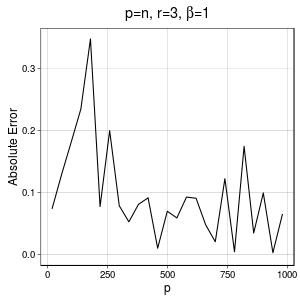
\includegraphics[height=6cm]{code/difference1.jpeg}
%    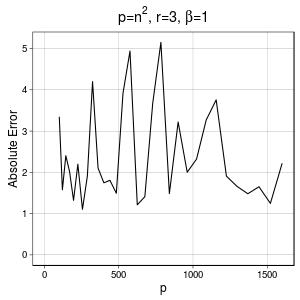
\includegraphics[height=6cm]{code/difference2.jpeg}\\
%    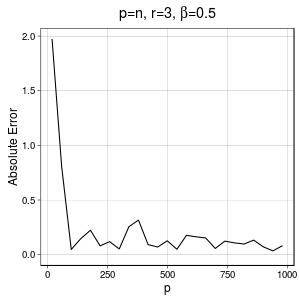
\includegraphics[height=6cm]{code/difference3.jpeg}
%    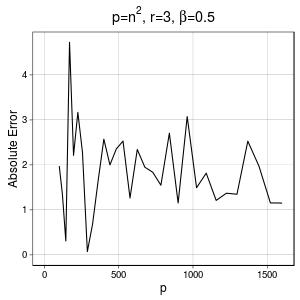
\includegraphics[height=6cm]{code/difference4.jpeg}\\
%    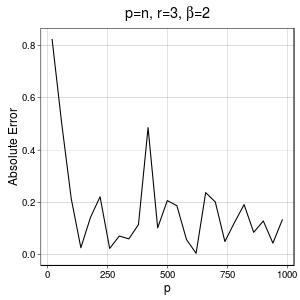
\includegraphics[height=6cm]{code/difference5.jpeg}
%    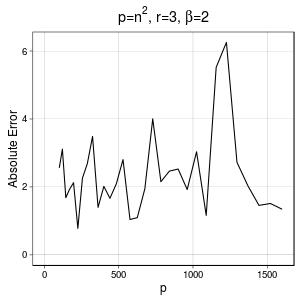
\includegraphics[height=6cm]{code/difference6.jpeg}\\
%    \caption{These are plots of $T_{\textrm{dif}}$ versus $p$. The first column and the second column are the case of $p=n$ and $p=n^2$, separately. The cases of $\beta=1,2,3$ are in the row $1,2,3$ separately. $r$ is set to be $3$ in all cases. }\label{fig:fig1}
%\end{figure}

First, we simulate the level of the new test. We set factor number $r=1$.
Samples are repeatedly generated $2000$ times to calculate empirical level.
For comparison, we also give the corresponding `oracle' level which is calculated by variable ${T_1}/(\sigma^2\sqrt{2p\tau^2})$.
The result is listed in
Table~\ref{biaoge1}.
Level of the new test is a little inflated compared with oracle level.

% latex table generated in R 3.3.1 by xtable 1.8-2 package
% Sun Jul 31 01:50:20 2016
\begin{table}[ht]
\caption{$n_1=n_2=60$} 
\label{hahaha}
\vspace{3mm}
\centering
\begin{tabular}{lllllllllllll}
\toprule
    &   \multicolumn{4}{c}{Normal} & \multicolumn{4}{c}{Chi-squared}& \multicolumn{4}{c}{Student's $t$}  \\
    \cmidrule(r){2-5}
\cmidrule(r){6-9}
\cmidrule(r){10-13}
    $p$ & $200$ & $400$ & $600$ & $800$ & $200$ & $400$ & $600$ & $800$ & $200$ & $400$ & $600$ & $800$ \\ 
\midrule
    $\beta=0.5$\\
New1 & 0.092 & 0.109 & 0.121 & 0.132 & 0.082 & 0.111 & 0.118 & 0.130 & 0.093 & 0.119 & 0.123 & 0.136 \\ 
New2 & 0.057 & 0.064 & 0.067 & 0.070 & 0.050 & 0.065 & 0.070 & 0.081 & 0.060 & 0.068 & 0.067 & 0.073 \\ 
oracle & 0.048 & 0.051 & 0.049 & 0.051 & 0.040 & 0.046 & 0.051 & 0.052 & 0.052 & 0.050 & 0.047 & 0.051 \\ 
chi & 0.046 & 0.045 & 0.044 & 0.035 & 0.043 & 0.045 & 0.041 & 0.042 & 0.042 & 0.040 & 0.036 & 0.040 \\ 
fast & 0.067 & 0.061 & 0.059 & 0.052 & 0.065 & 0.071 & 0.057 & 0.057 & 0.066 & 0.063 & 0.059 & 0.057 \\ 
CQ & 0.060 & 0.057 & 0.059 & 0.054 & 0.059 & 0.068 & 0.059 & 0.061 & 0.061 & 0.058 & 0.057 & 0.058 \\ 
    $\beta=1$\\
New1 & 0.094 & 0.107 & 0.134 & 0.148 & 0.099 & 0.114 & 0.134 & 0.136 & 0.081 & 0.113 & 0.137 & 0.140 \\ 
New2 & 0.061 & 0.071 & 0.081 & 0.090 & 0.070 & 0.072 & 0.074 & 0.067 & 0.056 & 0.068 & 0.086 & 0.076 \\ 
oracle & 0.051 & 0.056 & 0.063 & 0.059 & 0.054 & 0.059 & 0.051 & 0.046 & 0.046 & 0.051 & 0.059 & 0.052 \\ 
chi & 0.048 & 0.059 & 0.052 & 0.052 & 0.062 & 0.055 & 0.054 & 0.045 & 0.055 & 0.058 & 0.057 & 0.064 \\ 
fast & 0.050 & 0.053 & 0.050 & 0.056 & 0.060 & 0.054 & 0.056 & 0.043 & 0.058 & 0.058 & 0.058 & 0.061 \\ 
CQ & 0.067 & 0.074 & 0.068 & 0.072 & 0.084 & 0.067 & 0.072 & 0.065 & 0.075 & 0.081 & 0.080 & 0.086 \\ 
    $\beta=2$\\
New1 & 0.076 & 0.112 & 0.117 & 0.127 & 0.095 & 0.110 & 0.115 & 0.135 & 0.090 & 0.105 & 0.128 & 0.131 \\ 
New2 & 0.049 & 0.070 & 0.071 & 0.066 & 0.067 & 0.066 & 0.068 & 0.075 & 0.062 & 0.061 & 0.079 & 0.072 \\ 
oracle & 0.041 & 0.050 & 0.048 & 0.040 & 0.056 & 0.044 & 0.044 & 0.050 & 0.050 & 0.050 & 0.050 & 0.046 \\ 
chi & 0.056 & 0.057 & 0.055 & 0.058 & 0.056 & 0.059 & 0.061 & 0.046 & 0.048 & 0.048 & 0.058 & 0.058 \\ 
fast & 0.057 & 0.057 & 0.051 & 0.056 & 0.059 & 0.059 & 0.063 & 0.051 & 0.051 & 0.050 & 0.059 & 0.057 \\ 
 CQ & 0.076 & 0.072 & 0.067 & 0.079 & 0.072 & 0.077 & 0.082 & 0.067 & 0.070 & 0.065 & 0.079 & 0.080 \\ 
\bottomrule
\end{tabular}
\end{table}


% latex table generated in R 3.3.1 by xtable 1.8-2 package
% Sun Jul 31 01:50:20 2016
\begin{table}[ht]

\caption{Test level simulation. Equal variance case.} 
\label{biaoge1}
    \vspace{3mm}
\centering
\begin{tabular}{rccccccc}
    \toprule
     &  & \multicolumn{2}{c}{$\beta$=0.5} & \multicolumn{2}{c}{$\beta$=1}& \multicolumn{2}{c}{$\beta$=2}   \\
    \cmidrule(r){3-4}
    \cmidrule(r){5-6}
    \cmidrule(r){7-8}
$n$ & $p$ & NEW & ORACLE & NEW & ORACLE & NEW & ORACLE \\ 
\midrule
300 & 200 & 0.075 & 0.062 & 0.079 & 0.062 & 0.074 & 0.070 \\ 
  300 & 400 & 0.074 & 0.065 & 0.061 & 0.044 & 0.046 & 0.040 \\ 
  300 & 600 & 0.058 & 0.041 & 0.070 & 0.052 & 0.071 & 0.055 \\ 
  300 & 800 & 0.066 & 0.047 & 0.071 & 0.052 & 0.062 & 0.048 \\ 
  600 & 200 & 0.061 & 0.055 & 0.052 & 0.051 & 0.058 & 0.056 \\ 
  600 & 400 & 0.051 & 0.048 & 0.051 & 0.042 & 0.059 & 0.051 \\ 
  600 & 600 & 0.061 & 0.058 & 0.056 & 0.054 & 0.051 & 0.047 \\ 
  600 & 800 & 0.053 & 0.046 & 0.060 & 0.050 & 0.056 & 0.048 \\ 
   \bottomrule
\end{tabular}
\end{table}

%% latex table generated in R 3.3.3 by xtable 1.8-2 package
% Thu Jun  1 20:35:00 2017
\begin{table}[ht]

\caption{Test level simulation. Unequal variance case.} 
\label{biaoge2}
    \vspace{3mm}
\centering
\begin{tabular}{rccccccc}
  \toprule
    &  & \multicolumn{2}{c}{$\beta$=0.5} & \multicolumn{2}{c}{$\beta$=1}& \multicolumn{2}{c}{$\beta$=2}   \\
    \cmidrule(r){3-4}
    \cmidrule(r){5-6}
    \cmidrule(r){7-8}
$n$ & $p$ & NEW & ORACLE & NEW & ORACLE & NEW & ORACLE \\ 
\midrule
300 & 200 & 0.066 & 0.058 & 0.057 & 0.054 & 0.054 & 0.050 \\ 
  300 & 400 & 0.063 & 0.047 & 0.063 & 0.047 & 0.069 & 0.052 \\ 
  300 & 600 & 0.070 & 0.058 & 0.091 & 0.059 & 0.086 & 0.053 \\ 
  300 & 800 & 0.069 & 0.040 & 0.097 & 0.055 & 0.083 & 0.056 \\ 
  600 & 200 & 0.054 & 0.056 & 0.049 & 0.049 & 0.052 & 0.051 \\ 
  600 & 400 & 0.060 & 0.054 & 0.067 & 0.059 & 0.060 & 0.055 \\ 
  600 & 600 & 0.041 & 0.034 & 0.069 & 0.062 & 0.055 & 0.049 \\ 
  600 & 800 & 0.077 & 0.063 & 0.066 & 0.058 & 0.071 & 0.058 \\ 
   \bottomrule
\end{tabular}

\end{table}




Next, we simulate the empirical power of the new test.
The results in Section~\ref{sec:chen} have showed that the level of the~\cite{Chen2010A}'s test can't be guaranteed when $\beta\geq 1/2$.
To be fair,  critical values are all determined by permutation method.
%We set $\bSigma_1=\bSigma_2$, under which permutation method can produce exact test procedures, see~\cite{Lehmann}'s Example 15.2.2.\@
%Note that the statistics of~\cite{Chen2010A},~\cite{Bai1996Efiect} and~\cite{Ma2015A} all produce the same permutation test.
%Indeed, they are all equivalent to the permutation test based on $\|\bar{X}_1-\bar{X}_2\|^2$.
We permute the sample $100$ times to determine the critical value. The test procedure is repeated $500$ times to obtain empirical power.
We plot the empirical power versus signal-to-noise ratio (SNR) which is defined as $\textrm{SNR}=\|\mu_1-\mu_2\|^2/(\sigma^2\sqrt{2\tau^2 p})$.
The results are illustrated in figure~\ref{fig:fig1}, where `NEW', `CQ' and `SD' represent the new test,~\cite{Chen2010A}'s test and \cite{Srivastava2008A}'s test respectively.
From the results, we can find that when $\bSigma$ is spiked, the new test outperforms $T_{CQ}$ substantially; when $\bSigma$ is not spiked, all three tests have similar performance.
\begin{figure}
    \centering 
    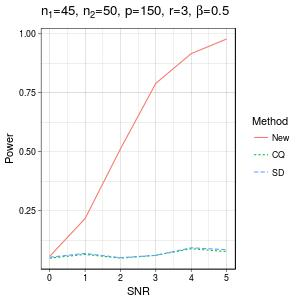
\includegraphics[height=6cm]{code/fig1.jpeg}
    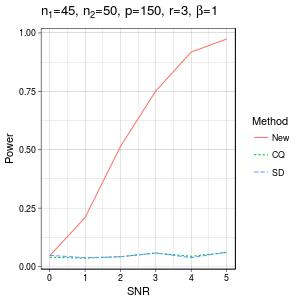
\includegraphics[height=6cm]{code/fig2.jpeg}
    \\
    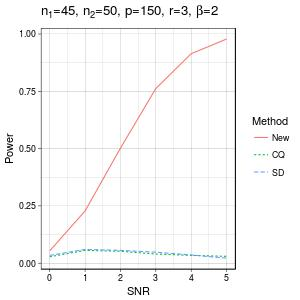
\includegraphics[height=6cm]{code/fig3.jpeg}
    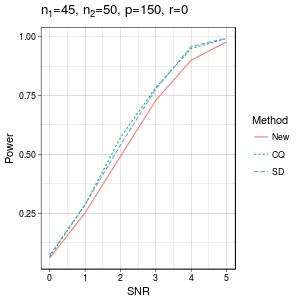
\includegraphics[height=6cm]{code/fig4.jpeg}
    \caption{Empirical power simulation.}\label{fig:fig1}
\end{figure}

\begin{figure}
    \centering 
    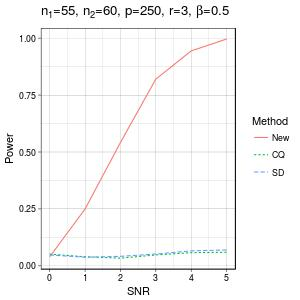
\includegraphics[height=6cm]{code/fig5.jpeg}
    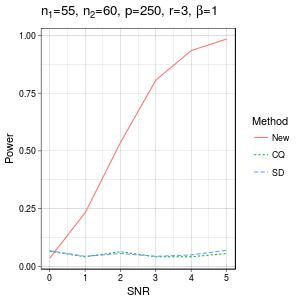
\includegraphics[height=6cm]{code/fig6.jpeg}
    \\
    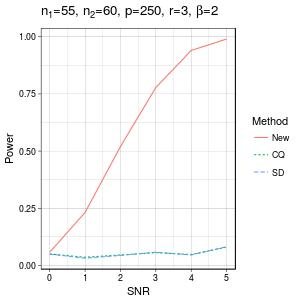
\includegraphics[height=6cm]{code/fig7.jpeg}
    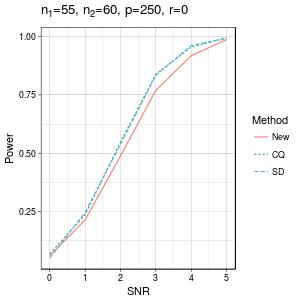
\includegraphics[height=6cm]{code/fig8.jpeg}
    \caption{Empirical power simulation.}\label{fig:fig2}
\end{figure}
%Permutation method is computation expensive. So when $p$ and $n$ are large, we simulate empirical power by asymptotic distribution. The results are illustrated in figure~\eqref{fig:fig3}.

%\begin{figure}\label{fig:fig3}
    %\centering 
    %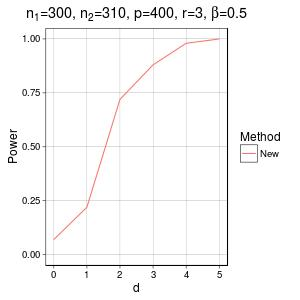
\includegraphics[height=6cm]{code/newfig1.jpeg}
    %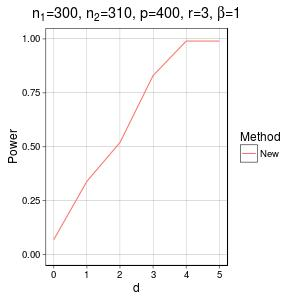
\includegraphics[height=6cm]{code/newfig2.jpeg}
    %\\
    %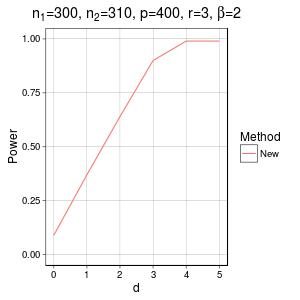
\includegraphics[height=6cm]{code/newfig3.jpeg}
    %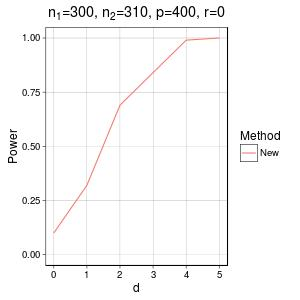
\includegraphics[height=6cm]{code/newfig4.jpeg}
    %\\
    %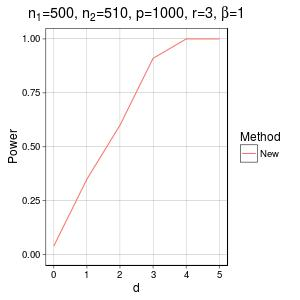
\includegraphics[height=6cm]{code/newfig5.jpeg}
    %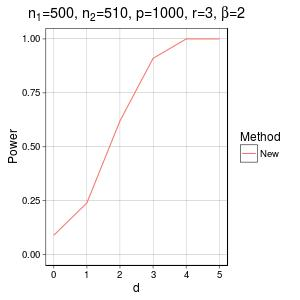
\includegraphics[height=6cm]{code/newfig6.jpeg}
    %\caption{Empirical Power (critical values are computed by asymptotic distribution)}\label{fig:fig3}
%\end{figure}

\subsection{Real data analysis}
In this section, we study the practical problem considered in~\cite{Ma2015A}.
The task is to test whether Monday stock returns are equal to those of other trading days on average.
Define an observation be the log return of stocks in a day.
Hence $p$ is the total number of stocks.
Let sample $1$ and sample $2$ be the observations on Monday and the other trading days, respectively.
Then we would like to test $H_0\, :\mu_1=\mu_2$ v.s. $H_1\,:\mu_1\neq \mu_2$.
We collected the data of $p=710$
 stocks of China
from 01/04/2013 to 12/31/2014. There are total $n_1=95$ Monday and $n_2=388$ other trading days. 

We assume $\bSigma_1=\bSigma_2$.
The first eigenvalue of $S$ is $0.14$, which is significantly larger than the others.
In fact, the second eigenvalue is $0.02$.
Hence there's clearly a spiked eigenvalue.
We set $r=1$ and perform our new test.
The $p$ value is $0.149$, which is obtained by $1000$ permutations.
Hence, the null hypothesis can not be rejected for $\alpha=0.05$.
We draw the same conclusion as~\cite{Ma2015A}.

\section{Conclusion remark}



This paper is concerned with the problem of testing the equality of means in the setting of high dimension and spiked covariance.
We derived the asymptotic distribution of~\cite{Chen2010A}'s test statistic.
To reduce the variance of $T_{CQ}$, we dropped big variance terms and obtain a new test statistic. The asymptotic normality of the new statistic is proved and the asymptotic power is given. %The new test outperforms $T_{CQ}$ substantially if the variance is spiked.

%We also generalize the test to unequal variance case.

In another paper,~\cite{Zhao2016A} proved that their test statistic can be written in the form of projection. Their simulation results showed that their test performs well under strong correlations.
Our work partially explains why their test performs well although the projections are slightly different. 

 Spiked covariance is an important correlation pattern and has been widely studied in terms of PCA\@.
 In PCA, authors focus on the principal subspace.
 However, in some circumstances, as our work have shown, the complement of principal subspace is more useful. 

In our paper, we have assumed $r$ is known. If $r$ is an unknown positive number, a consistent estimator of $r$ is
\begin{equation}\label{estimateR}
    \hat{r}=\textrm{argmax}_{l\leq R}\frac{\lambda_l(S)}{\lambda_{l+1}(S)},
\end{equation}
where $R$ is a hyperparameter.
    See~\cite{Ahn2009Eigenvalue} for detail.


The asymptotic normality of the new test statistic relies on the assumption $\sqrt{p}/n\to 0$. In the situation of small $n$ or very large $p$, the critical value of the new test can be determined by permutation method. Our simulation shows that the new test still performs well. It remains a theoretical interest to study the asymptotic behavior of permutation based test in these situations.

{\color{red}
Non normality
}


\section*{Appendix}
%We denote by $\|\cdot \|$ and $\|\cdot\|_F$ the operator and Frobenius  norm of matrix, respectively.

%\begin{lemma}\label{lemma1}
%    let $X$ be a $p$-dimensional random vector with distribution $N(0,\bSigma)$. Denote the spectral decomposition of $\bSigma$ by $\bSigma =\sum_{i=1}^p \lambda_i p_i p_i^T$ with $\lambda_1\geq \cdots \geq \lambda_p$. Then $X^T p_i p_i^T X$ is stochastically larger than $X^T p_j p_{j}^T X$ for $i<j$.
%\end{lemma}
%\begin{proof}[\textbf{Proof}]
%    The lemma is established immediately once we note that $X^T p_i p_i^T X/\sqrt{\lambda_i}$ is distributed as $\chi^2$ distribution with freedom $1$.
%\end{proof}

\begin{lemma}[Weyl's inequality]
Let $H$ and $P$ be two symmetric $n\times n$ matrices and $M=H+P$. If $r+s-1 \leq  i\leq j+k-n$, we have
\begin{equation*}
\lambda_j(H)+\lambda_k(P)\leq \lambda_i(M) \leq \lambda_r(H)+\lambda_s(P).
\end{equation*}
    See, for example,~\cite{Horn1985Matrix} Theorem $4.3.1$.
\end{lemma}
%\begin{corollary}\label{WeylCor}
    %Let $H$ and $P$ be two symmetric matrices and $M=H+P$. If $\mathrm{rank}(P)< k\leq n$, then
    %\begin{equation*}
        %\lambda_k(M)\leq \lambda_1(H).
    %\end{equation*}
%\end{corollary}

{\color{red}
\begin{lemma}[\cite{Cai2015Optimal}, Proposition 1]\label{pert}
    Let $A_1$ and $A_2$ be $p\times p$ symmetric matrices. Let $r<p$ be arbitrary and let $\BV_1, \BV_2\in \mathbb{O}_{p,r}$ be formed by the $r$ leading singular vectors of $A_1$ and $A_2$, respectively. Then
    $$
    \|A_1-A_2\|\geq \frac{1}{2}(\lambda_r(A_1)-\lambda_{r+1}(A_2))\|\BV_1 \BV_1^T- \BV_2 \BV_2^T\|.
    $$
\end{lemma}
}




{\color{red}
    \begin{lemma}[\cite{DAVIDSON2001317}, Theorem II.7]\label{DSbound}
        Let $Z$ be a $p\times n$ random matrix with i.i.d. $N(0,1)$ entries.
        Then for any $t>0$,
        \begin{align*}
            &\Pr(\sqrt{\lambda_1(Z Z^T )}>\sqrt{n}+\sqrt{p}+t)\leq e^{-t^2/2},
            \\
            &\Pr(\sqrt{\lambda_{\min(n,p)}(Z Z^T )}<\sqrt{n}-\sqrt{p}-t)\leq e^{-t^2/2}.
        \end{align*}
    \end{lemma}
    We give two useful corollaries of Lemma~\ref{DSbound}.
}
\begin{corollary}\label{maxEigen}
    Suppose that $W_n$ is a $p \times p$ random matrix distributed as $\mathrm{Wishart}_p(n,\BI_{p})$, the $p$ dimensional Wishart distribution with parameter $\Psi$ and $m$ degrees of freedom. Then as $n,p\to \infty$,
    $$
        \lambda_1(W_n)=O_P(\max(n,p)).
    $$
\end{corollary}
{\color{red}
\begin{proof}[\textbf{Proof}]
    The result follows from the inequality
    $$
    \begin{aligned}
        &\Pr\Big(\frac{\lambda_1(W_n)}{\max(n,p)}>16\Big)
        \leq
        \Pr\Big(\lambda_1(W_n)>8(n+p)\Big)
        \leq
        \Pr\Big(\lambda_1(W_n)>4(\sqrt{n}+\sqrt{p})^2\Big)\\
        =
        &\Pr\Big(\sqrt{\lambda_1(W_n)}>2(\sqrt{n}+\sqrt{p})\Big)
        \leq
        \Pr\Big(\sqrt{\lambda_1(W_n)}>2\sqrt{n}+\sqrt{p}\Big)\leq e^{-n/2},
    \end{aligned}
    $$
    where the last inequality follows from Lemma~\ref{DSbound} with $t=\sqrt{n}$.
\end{proof}
}

{\color{red}
\begin{corollary}\label{corNorm}
Suppose that $W_n$ is a $p \times p$ random matrix distributed as $\mathrm{Wishart}_p(n,\BI_{p})$. Then as $n,p\to \infty$,
$$
    \|\frac{1}{n}W_n-\BI_p\|=O_P\Big(\max\big(\sqrt{\frac{p}{n}},\frac{p}{n}\big)\Big).
$$
\end{corollary}
\begin{proof}
    Since the eigenvalues of $\frac{1}{n}W_n-\BI_p$ are $\frac{1}{n}\lambda_1(W_n)-1\geq\cdots\geq\frac{1}{n}\lambda_p(W_n)-1$, we have
     $$\|\frac{1}{n}W_n-\BI_p\|=\max\Big(\frac{1}{n}\lambda_1(W_n)-1,1-\frac{1}{n}\lambda_p(W_n)\Big).$$
This, combined with union bound, yields
$$
    \Pr\Big(\|\frac{1}{n}W_n-\BI_p\|>4\big(\sqrt{\frac{p}{n}}+\frac{p}{n}\big)\Big)
    \leq
    \Pr\Big(\lambda_1(W_n)>\big(\sqrt{n}+2\sqrt{p}\big)^2\Big)+
    \Pr\Big(\lambda_p(W_n)<n-4\sqrt{np}-4p\Big).
$$
    The first term can be bounded by Lemma~\ref{DSbound} with $t=\sqrt{p}$.
    $$
    \Pr\Big(\lambda_1(W_n)>\big(\sqrt{n}+2\sqrt{p}\big)^2\Big)=
    \Pr\Big(\sqrt{\lambda_1(W_n)}>\sqrt{n}+2\sqrt{p}\Big)\leq e^{-p^2/2}.
    $$
    We now show that the second term is also bounded by $e^{-p^2/2}$.
    To see this, note that
    If $p>n/4$, then $n-4\sqrt{np}-4p\leq n-4p<0$. In this case, $\Pr\Big(\lambda_p(W_n)<n-4\sqrt{np}-4p\Big)=0$.
    If $p\leq n/4$, we have
    $$
    \begin{aligned}
        &\Pr\Big(\lambda_p(W_n)<n-4\sqrt{np}-4p\Big)
    \leq
    \Pr\Big(\lambda_p(W_n)<n-4\sqrt{np}+4p\Big)\\
        =&
    \Pr\Big(\sqrt{\lambda_p(W_n)}<\sqrt{n}-\sqrt{2p}\Big)
        \leq e^{-p^2/2},
    \end{aligned}
    $$
    where the last inequality follows from Lemma~\ref{DSbound} with $t=\sqrt{p}$.

    Now we have the bound
    $$
    \Pr\Big(\|\frac{1}{n}W_n-\BI_p\|>4\big(\sqrt{\frac{p}{n}}+\frac{p}{n}\big)\Big)
    \leq 2 e^{-p^2/2}.
    $$
    Then 
    $$\|\frac{1}{n}W_n-\BI_p\|=O_P\Big(\sqrt{\frac{p}{n}}+\frac{p}{n}\Big)=O_P\Big(\max\big(\sqrt{\frac{p}{n}},\frac{p}{n}\big)\Big).$$
\end{proof}
}


\begin{proof}[\textbf{Proof of Lemma~\ref{quadraticFormCLT}}]
    By a standard orthogonal transformation, we can write
    \begin{equation}
        \frac{Y_n^T \BA_n Y_n-\myE Y_n^T \BA_n Y_n}{{[\myVar(Y_n^T \BA_n Y_n)]}^{1/2}}=\sum_{i=1}^{k_n}\frac{\lambda_i(\BA_n)}{{\big[2\mytr(\BA_n^2)\big]}^{1/2}}(Z_{ni}^2-1),
    \end{equation}
    where $Z_{n1},\ldots,Z_{n k_n}$ are independent standard normal random variables.

    If~\ref{quadraticEigen} holds, then
    \begin{equation*}
        \begin{aligned}
            &\sum_{i=1}^{k_n}\myE\Big[\frac{\lambda_i^2(\BA_n)}{2\mathrm{tr}(\BA_n^2)}{(Z_{ni}^2-1)}^2\Big\{\frac{\lambda_i^2(\BA_n)}{2\mathrm{tr}(\BA_n^2)}{(Z_{ni}^2-1)}^2\geq \epsilon\Big\}\Big]\\
            \leq&\sum_{i=1}^{k_n}
            \frac{\lambda_i^2(\BA_n)}{2\mytr(\BA_n^2)}
            \myE\Big[{(Z_{n1}^2-1)}^2\Big\{\frac{\lambda_{1}(\BA_n^2)}{2\mytr(\BA_n^2)}{(Z_{n1}^2-1)}^2\geq \epsilon\Big\}\Big]\\
            =&
            \frac{1}{2}\myE\Big[{(Z_{n1}^2-1)}^2\Big\{\frac{\lambda_{1}(\BA_n^2)}{2\mytr(\BA_n^2)}{(Z_{n1}^2-1)}^2\geq \epsilon\Big\}\Big]\to 0.
        \end{aligned}
    \end{equation*}
    Hence~\ref{quadratic} follows by Lindeberg's central limit theorem.

    Conversely, if~\ref{quadratic} holds, we will prove that there is a subsequence of $\{n\}$ along which~\ref{quadraticEigen} holds. Then~\ref{quadraticEigen} follows by a standard contradiction argument. 

    Denote $c_{ni}=\lambda_i(\BA_n)/{\big[2\mytr(\BA_n^2)\big]}^{1/2}$, $i=1,\ldots,k_n$.
    Since~\ref{quadratic} holds, the characteristic function of
        $
        \sum_{i=1}^{k_n}c_{ni}(Z_{ni}^2-1)
    $
    converges to $\exp(-t^2/2)$ for every $t$.
    Denote by $\log z$ $(z\in\mathbb{C})$ the principal branch of the complex logarithm.
    For $t\in (-1/2,1/2)$, we have
    \begin{equation*}
        \begin{aligned}
            &\myE\big[\exp{\big(it \sum_{j=1}^{k_n}c_{nj}(Z_{nj}^2-1)\big)}\big]
            =
            \exp\Big(-i(\sum_{j=1}^{k_n}c_{nj})t-
            \frac{1}{2}\sum_{j=1}^{k_n}\log(1-i2c_{nj}t) \Big)\\
            =&
            \exp\Big(
            -i(\sum_{j=1}^{k_n}c_{nj})t+
            \frac{1}{2}\sum_{j=1}^{k_n}\sum_{l=1}^{+\infty}\frac{1}{l}{(i2c_{nj}t)}^l
            \Big)
            =
            \exp\Big(
            -i(\sum_{j=1}^{k_n}c_{nj})t+
            \frac{1}{2}\sum_{l=1}^{+\infty}\Big[\sum_{j=1}^{k_n}{(c_{nj})}^l\Big]\frac{1}{l}{(i2t)}^l\Big)\\
            =&
            \exp\Big(
            -\frac{1}{2}t^2+
            \frac{1}{2}\sum_{l=3}^{+\infty}\Big[\sum_{j=1}^{k_n}{(c_{nj})}^l\Big]\frac{1}{l}{(i2t)}^l \Big),
        \end{aligned}
    \end{equation*}
    where the second equality holds since $0\leq c_{ni}\leq \sqrt{2}/2$ by definition.
    Let $b_{nl}=\sum_{j=1}^{k_n}{(c_{nj})}^l$, $n=1,2,\cdots$ and $l=3,4,\cdots$.
    Note that for $l\geq 3$, we have
    $$|b_{nl}|=\big|\sum_{j=1}^{k_n}{(c_{nj})}^l\big|\leq \big|\sum_{j=1}^{k_n}{(c_{nj})}^2\big|=1/2.$$
    By Helly's selection theorem, there's a subsequence of $\{n\}$ along which $\lim_{n\to \infty}b_{nl}=b_l$ exists for every $l$.
    For this subsequence, applying dominated convergence theorem yields
            $$\myE \big[\exp{\big(it \sum_{j=1}^{k_n}c_{nj}(Z_{nj}^2-1)\big)}\big]
            \to
            \exp\Big(
            -\frac{1}{2}t^2+
            \frac{1}{2}\sum_{l=3}^{+\infty}b_l\frac{1}{l}{(i2t)}^l\Big),
            \quad t\in\big(-\frac{1}{2},\frac{1}{2}\big).
            $$
            But the left hand side converges to $\exp(-t^2/2)$.
            It follows that
            $$
            -\frac{1}{2}t^2+
            \frac{1}{2}\sum_{l=3}^{+\infty}b_l\frac{1}{l}{(i2t)}^l
            =-\frac{1}{2}t^2+ 2\pi m i,
            \quad t\in\big(-\frac{1}{2},\frac{1}{2}\big),
            $$
            for some integer $m$.
            By the uniqueness of power series, we mulst have $m=0$ and $b_l=0$ for $l\geq 3$. Then~\ref{quadraticEigen} follows by noting that $b_{n4}\geq \max_j{(c_{nj})}^4$.
\end{proof}





\begin{proof}[\textbf{Proves of Theorem~\ref{Chenstheory1} and Theorem~\ref{Chenstheory2}}]
    In both Theorem~\ref{Chenstheory1} and Theorem~\ref{Chenstheory2}, (a) is a corrolary of (b).
    Hence we shall prove (b) of Theorem~\ref{Chenstheory1} and Theorem~\ref{Chenstheory2} simultaneously.

For random variable $\xi$ and $\eta$,
  we write $\xi\sim \eta$ to denote they have the same distribution.
    Since $(n_k-1)S_k\sim \text{Wishart}_p(n_k-1,\bSigma)$, $k=1,2$, we have %$(n_1-1)\mytr S_1\sim \sum_{i=1}^{p} \lambda_i (\bSigma) W_i$ where $W_i\sim \chi^2_{n_1-1} $.
    %Note that $\lambda_{r+1}(\bSigma)=\cdots=\lambda_p(\bSigma)=\sigma^2$, by central limit theorem, we have
    %$$
    %\begin{aligned}
        %&\sum_{i=1}^{p} \lambda_i (\bSigma) W_i=
    %\sum_{i=1}^{r} \lambda_i (\bSigma) W_i+
    %\sum_{i=r+1}^{p} \sigma^2 W_i\\
        %\sim&
    %\sum_{i=1}^{r} \lambda_i (\bSigma) W_i+
        %(p-r)(n_1-1)\sigma^2+
        %\sqrt{(n_1-1)(p-r)}\sigma^2\epsilon+o_P(\sqrt{np}),
    %\end{aligned}
    %$$
    %where $\epsilon\sim N(0,1)$. By law of large numbers, we have $W_i/(n_i-1)\xrightarrow{P}1$. Hence
%$$
%\begin{aligned} 
    %\frac{1}{\tau p^{\beta} n_1}\mytr S_1
    %&\sim
    %\frac{1}{\tau n_1}\sum_{i=1}^{r} \frac{\lambda_i +\sigma^2}{p^{\beta}} \frac{W_i}{n_i-1}+
        %\frac{p-r}{\tau p^{\beta}n_1}\sigma^2+
        %\frac{1}{\tau p^\beta n_1}\sqrt{\frac{p-r}{n_1-1}}\sigma^2\epsilon+o_P(n^{-1/2}p^{1/2-\beta})\\
        %&=
    %\frac{1}{\tau n_1}\sum_{i=1}^{r} l_i+
        %\frac{p-r}{\tau p^{\beta}n_1}\sigma^2+
        %\frac{1}{\tau p^\beta n_1}\sqrt{\frac{p-r}{n_1-1}}\sigma^2\epsilon+o_P(1)\\
%\end{aligned}
%$$
%
    %Hence
    $$
 \myE\Big(\frac{1}{n_1}\mytr S_1+\frac{1}{n_2}\mytr S_2\Big)=\tau \mytr\bSigma,
    $$
    and
    $$
    \begin{aligned}
        &\myVar\Big(\frac{1}{n_1}\mytr S_1+\frac{1}{n_2}\mytr S_2\Big)=
        \Big(\frac{2}{n_1^2(n_1-1)}+\frac{2}{n_2^2(n_2-1)}\Big)\mytr \bSigma^2\\
        =&
    O\Big(\frac{1}{n^3}(p^{2\beta}+p)\Big)=O\Big(\frac{p^{2\beta}}{n^3}\Big).
    \end{aligned}
    $$
    It follows that
    $$
    \begin{aligned}
        &\frac{1}{n_1}\mytr S_1+\frac{1}{n_2}\mytr S_2=
    \tau \mytr \bSigma+O_P\Big(\frac{1}{n\sqrt{n}}p^{\beta}\Big)\\
        =&\tau \sum_{i=1}^r (\lambda_i+\sigma^2)+\tau(p-r)\sigma^2+O_P\Big(\frac{1}{n\sqrt{n}}p^{\beta}\Big)\\
        =&\tau p^{\beta} \sum_{i=1}^r \omega_i+\tau(p-r)\sigma^2+o_P\Big(\frac{1}{n}p^{\beta}\Big).
    \end{aligned}
    $$
Thus,
        \begin{equation}\label{eq:kkk1}
        \frac{1}{\tau p^\beta}\big(\frac{1}{n_1}\mytr S_1+\frac{1}{n_2}\mytr S_2\big)
        =\sum_{i=1}^r \omega_i+p^{1-\beta}\sigma^2+o_P(1).
        \end{equation}

    Next we deal with $\|\bar{X}_1-\bar{X}_2\|^2$.
    Note that we have
    $$
    \|\bar{X}_1-\bar{X}_2\|^2=
    \|\BV^T(\bar{X}_1-\bar{X}_2)\|^2+
    \|\tilde{\BV}^T(\bar{X}_1-\bar{X}_2)\|^2.
    $$
    These two terms are independent.
    For the first term, note that $\BV^T(\bar{X}_1-\bar{X}_2)\sim N_r\big(\BV^T (\mu_1-\mu_2),\tau (\bLambda+\sigma^2 \BI_r)\big)$, we have
    $$
    \begin{aligned}
        \|\BV^T(\bar{X}_1-\bar{X}_2)\|^2&\sim
        \sum_{i=1}^r \Big(\sqrt{\tau (\lambda_i+\sigma^2)}Z_i+\big(\BV^T (\mu_1-\mu_2)\big)_i \Big)^2\\
        &=\tau p^{\beta}
        \sum_{i=1}^r
        \Big( \sqrt{p^{-\beta}(\lambda_i+\sigma^2)}Z_i+\frac{1}{\sqrt{\tau p^{\beta}}}\big(\BV^T (\mu_1-\mu_2)\big)_i \Big)^2.
    \end{aligned}
    $$
    By the assumptions of the theorem,  we have that
    \begin{equation}\label{eq:kkk2}
    \begin{aligned}
        \frac{1}{\tau p^{\beta}}\|\BV^T(\bar{X}_1-\bar{X}_2)\|^2
        \xrightarrow{w}
        \sum_{i=1}^r (\sqrt{\omega_i} Z_i+\zeta_i)^2.
    \end{aligned}
    \end{equation}

    As for $\|\tilde{\BV}^T(\bar{X}_1-\bar{X}_2)\|^2$, we have that
        $$
        \begin{aligned}
            &\|\tilde{\BV}^T(\bar{X}_1-\bar{X}_2)\|^2
            =\big\|\tilde{\BV}^T(\mu_1-\mu_2)+\tilde{\BV}^T\big((\bar{X}_1-\mu_1)-(\bar{X}_2-\mu_2)\big)\big\|^2\\
            =&\|\tilde{\BV}^T(\mu_1-\mu_2)\|^2+
            \big\|\tilde{\BV}^T\big((\bar{X}_1-\mu_1)-(\bar{X}_2-\mu_2)\big)\big\|^2+
            2{(\mu_1-\mu_2)}^T\tilde{\BV}\tilde{\BV}^T\big((\bar{X}_1-\mu_1)-(\bar{X}_2-\mu_2)\big).
        \end{aligned}
        $$
Since $\tilde{\BV}^T (\bar{X}_1-\bar{X}_2)\sim N_{p-r}(\tilde{\BV}^T (\mu_1-\mu_2),  \sigma^2 \tau \BI_{p-r})$, by central limit theorem, we have
    $$
\frac{
    \big\|\tilde{\BV}^T\big((\bar{X}_1-\mu_1)-(\bar{X}_2-\mu_2)\big)\big\|^2-\sigma^2 \tau (p-r)}{\sigma^2 \tau\sqrt{2(p-r)}}\xrightarrow{\mathcal{L}} N(0,1).
    $$
    For the intersection term, we have
    \begin{equation*}
        \begin{aligned}
            &2{(\mu_1-\mu_2)}^T\tilde{\BV}\tilde{\BV}^T\big((\bar{X}_1-\mu_1)-(\bar{X}_2-\mu_2)\big)
            \sim N(0,4\sigma^2 \tau \|\tilde{\BV}^T(\mu_1-\mu_2)\|^2)\\
            =& O_P(\sqrt{\tau}\|\tilde{\BV}^T(\mu_1-\mu_2)\| )=o_P(\tau p^{\beta}).
        \end{aligned}
    \end{equation*}
    It follows that
    \begin{equation}\label{eq:kkk3}
\frac{1}{\tau p^\beta}
    \big(\big\|\tilde{\BV}^T(\bar{X}_1-\bar{X}_2)\big\|^2-\sigma^2 \tau (p-r)-\big\|\tilde{\BV}^T(\mu_1-\mu_2)\big\|^2\big)
    \xrightarrow{\mathcal{L}} 
        \sqrt{2}\sigma^2 \delta_{\{\frac{1}{2}\}}(\beta)Z_0,
    \end{equation}
    where $\delta_{\frac{1}{2}}(\beta)$ equals $1$ if $\beta=1/2$ and equals $0$ otherwise.


    Combining~\eqref{eq:kkk1}~\eqref{eq:kkk2} and~\eqref{eq:kkk3} leads to
    $$
    \begin{aligned}
        &\frac{1}{\tau p^{\beta}} T_{CQ}
        =\frac{1}{\tau p^{\beta}}\big(\|\bar{X}_1-\bar{X}_2\|^2-\frac{1}{n_1}\mytr S_1-\frac{1}{n_2}\mytr S_2\big)\\
        =&
        \frac{1}{\tau p^{\beta}}{\|\BV^T(\bar{X}_1-\bar{X}_2)\|^2}+
        \frac{1}{\tau p^{\beta}} \big({\|\tilde{\BV}^T(\bar{X}_1-\bar{X}_2)\|^2-\sigma^2 \tau(p-r)-\|\tilde{\BV}^T(\mu_1-\mu_2)\|^2}\big)\\
        &-\frac{1}{\tau p^{\beta}}\Big(\frac{1}{n_1}\mytr S_1+\frac{1}{n_2}\mytr S_2\Big)+\frac{\sigma^2 (p-r)}{p^\beta}+\frac{1}{\tau p^\beta}\|\tilde{\BV}^T(\mu_1-\mu_2)\|^2\\
        =&
        \sum_{i=1}^r (\sqrt{\omega_i} Z_i+\zeta_i)^2+
   \sqrt{2} \sigma^2 \delta_{\{\frac{1}{2}\}}(\beta)Z_0
        -
        (\sum_{i=1}^r \omega_i+p^{1-\beta}\sigma^2)
        +\frac{\sigma^2 (p-r)}{p^\beta}+\zeta^*+o_P(1)\\
        \xrightarrow{\mathcal{L}}&
        \sum_{i=1}^r (\sqrt{\omega_i} Z_i+\zeta_i)^2+
\zeta^*+
    \sqrt{2}\sigma^2 \delta_{\{\frac{1}{2}\}}(\beta)Z_0
        -
        \sum_{i=1}^r \omega_i.
    \end{aligned}
    $$
    This implies the conclusions of Theorem~\ref{Chenstheory1} and Theorem~\ref{Chenstheory2}.

    %Note that we have $\|\bar{X}_1-\bar{X}_2\|^2\sim \tau(\sum_{i=1}^r \lambda_i(\bSigma)Z_i+\sigma^2 W)$, where $Z_i\overset{i.i.d.}{\sim}\chi^2_1$ and $W\sim \chi^2_{p-r}$ is independent of $Z_i$'s. Then
    %$$
    %\frac{1}{\tau p^{\beta}}\|\bar{X}_1-\bar{X}_2\|^2
    %\sim\sum_{i=1}^r\frac{\lambda_i+\sigma^2}{p^{\beta}}Z_i
    %+\frac{\sigma^2}{p^{\beta}}W.
    %$$
    %It's easy to see that 
    %$$\sum_{i=1}^r\frac{\lambda_i+\sigma^2}{p^{\beta}}Z_i\xrightarrow{\mathcal{L}}\sum_{i=1}^r l_i Z_i.$$
    %By central limit theorem, we have
    %$$
    %\frac{1}{\sqrt{2(p-r)}}\big( W-(p-r)\big)\xrightarrow{\mathcal{L}}N(0,1).
    %$$
%
    %If $\beta=1/2$, by Slutsky's theorem we have
    %$$
    %\frac{1}{\tau p^{\beta}}\|\bar{X}_1-\bar{X}_2\|^2-\frac{\sigma^2(p-r)}{p^\beta}\xrightarrow{\mathcal{L}}
    %\sum_{i=1}^r l_i Z_i+\sqrt{2}\sigma^2 \epsilon.
    %$$
    %where $\epsilon\sim N(0,1)$

\end{proof}

\begin{proof}[\textbf{Proof of Proposition~\ref{eigenconsis}}]
    Let $\bSigma=\BU\BE\BU^T$ denote the spectral decomposition of $\bSigma$, where
     $\BU=(\BV,\tilde{\BV})$ and $\BE=\mydiag(\lambda_1+\sigma^2,\ldots,\lambda_r+\sigma^2,\sigma^2,\ldots,\sigma^2)$.
Denote by $S=\hat{\BU}\hat{\BE}\hat{\BU}^T$ the spectral decomposition of $S$, where $\hat{\BU}=(\hat{\BV},\hat{\tilde{\BV}})$ and $\hat{\BE}=\mydiag(\hat{\lambda}_1,\ldots,\hat{\lambda}_p)$.
Let $\bZ$ be a $p\times (n-2)$ random matrix with i.i.d. $N(0,1)$ entries.
Denote $\bZ={(\bZ_{(1)}^T,\bZ_{(2)}^T)}^T$, where $\bZ_{(1)}$ and $\bZ_{(2)}$ are the first $r$ rows and last $p-r$ rows of $\bZ$. 

    {\color{red}
The sample covariance matrix $S$ has the same distribution as
$
    {(n-2)}^{-1} \BU \BE^{1/2} \bZ \bZ^T \BE^{1/2} \BU^T
$.
This implies that $\hat{\lambda}_i=\lambda_i(S)\sim (n-2)^{-1}\lambda_i(\bZ^T \BE \bZ)$, $i=1,\ldots,r$.
Hence we only need to deal with the asymptotic property of $(n-2)^{-1}\lambda_i(\bZ^T \BE \bZ)$.
For $i=1,\ldots,r$, we have
    \begin{equation*}
        \begin{aligned}
            &|\lambda_i(\bZ^T \BE \bZ)-(n-2)(\lambda_i +\sigma^2)|\\
            \leq&
            |\lambda_i(\bZ^T \BE \bZ)-\lambda_i \big(\bZ_{(1)}^T(\bLambda+\sigma^2 \BI_r)\bZ_{(1)}\big)|
            +
|\lambda_i \big(\bZ_{(1)}^T(\bLambda+\sigma^2 \BI_r)\bZ_{(1)}\big)
        -(n-2)(\lambda_i +\sigma^2)|\\
        \end{aligned}
    \end{equation*}
    By the equality
$
    \bZ^T \BE \bZ= \bZ_{(1)}^T (\bLambda +\sigma^2 \BI_r) \bZ_{(1)}+
\sigma^2 \bZ_{(2)}^T  \bZ_{(2)}
$
and Weyl's inequality, the first term satisfies
$$
            |\lambda_i(\bZ^T \BE \bZ)-\lambda_i \big(\bZ_{(1)}^T(\bLambda+\sigma^2 \BI_r)\bZ_{(1)}\big)|
            \leq \|\bZ^T \BE \bZ-\bZ_{(1)}^T(\bLambda+\sigma^2 \BI_r)\bZ_{(1)}\|
            =\sigma^2\|\bZ_{(2)}^T  \bZ_{(2)}\|
    $$
For the second term, we have
$$
    \begin{aligned}
        &|\lambda_i \big(\bZ_{(1)}^T(\bLambda+\sigma^2 \BI_r)\bZ_{(1)}\big)-(n-2)(\lambda_i +\sigma^2)|\\
        =&
    \big|\lambda_i \big((\bLambda+\sigma^2 \BI_r)^{1/2}\bZ_{(1)}\bZ_{(1)}^T(\bLambda+\sigma^2 \BI_r)^{1/2}\big)
        -\lambda_i\big((n-2)(\bLambda+\sigma^2 \BI_r)\big)\big|\\
        \leq &
        \|
     (\bLambda+\sigma^2 \BI_r)^{1/2}\bZ_{(1)}\bZ_{(1)}^T(\bLambda+\sigma^2 \BI_r)^{1/2}
        -(n-2)(\bLambda+\sigma^2 \BI_r)
        \|\\
        \leq &
        (n-2)(\lambda_1 + \sigma^2)\big\|\frac{1}{n-2}\bZ_{(1)}\bZ_{(1)}^T-\BI_r\big\|,
    \end{aligned}
    $$
    where the first inequality follows from Weyl's inequality.
    Hence,
        $$
        \begin{aligned}
            &\Big|\frac{(n-2)^{-1}\lambda_i(\bZ^T \BE \bZ)}{\lambda_i}-1\Big|
            \leq \frac{1}{(n-2)\lambda_i}\Big|\lambda_i(\bZ^T \BE \bZ)-(n-2)(\lambda_i+\sigma^2)\Big|+\frac{\sigma^2}{\lambda_i}\\
            \leq&\frac{\sigma^2}{(n-2)\lambda_i}\|\bZ_{(2)}^T \bZ_{(2)}\|+\frac{\lambda_1+\sigma^2}{\lambda_i}\big\|\frac{1}{n-2}\bZ_{(1)}\bZ_{(1)}^T-\BI_r\big\|\Big)+\frac{\sigma^2}{\lambda_i}.
        \end{aligned}
        $$
        By Corollary~\ref{maxEigen}, the first term satisfies
        $$
        \frac{\sigma^2}{(n-2)\lambda_i}\|\bZ_{(2)}^T \bZ_{(2)}\|
        =O_P\Big(\max\big(\frac{\sigma^2}{\lambda_i},\frac{\sigma^2 p}{(n-2)\lambda_i}\big)\Big)=o_P(1).
        $$
        By law of large numbers, $\big\|\frac{1}{n-2}\bZ_{(1)}\bZ_{(1)}^T-\BI_r\big\|=o_P(1)$. Hence
        $$
            \Big|\frac{(n-2)^{-1}\lambda_i(\bZ^T \BE \bZ)}{\lambda_i}-1\Big|=o_P(1).
        $$
}

\end{proof}

\begin{lemma}\label{conRateLemma}
    Under Assumption~\ref{theModel}, we have
\begin{equation*}
\|\hat{\BV}\hat{\BV}^T-\BV\BV^T\|^2 =O_P(\frac{p}{p^{\beta}n}).
\end{equation*}
\end{lemma}
The convergence rate $p/(p^{\beta}n)$ is optimal, see~\cite{Cai2012Sparse}, Theorem 5.
{\color{red}
\begin{proof}[\textbf{Proof}]
    By Lemma~\ref{pert},
    $$
    \|\hat{\BV}\hat{\BV}^T - \BV\BV ^T\|\leq \frac{2}{\lambda_r}\|S-\bSigma\|.
    $$
    We only need to bound the right hand side
    Define $\BU$, $\BE$, $\bZ$, $\bZ_{(1)}$ and $\bZ_{(2)}$ as in the proof of Proposition~\ref{eigenconsis}.
    Since $S\sim (n-2)^{-1}\BU\BE^{1/2}\bZ \bZ^T \BE^{1/2} \BU^T$, we have
    $$
    \begin{aligned}
        &\|S-\bSigma\|=
        \|(\BV\BV^T+\tilde{\BV}\tilde{\BV}^T)(S-\bSigma)(\BV\BV^T+\tilde{\BV}\tilde{\BV}^T)\|\\
        \leq& \|\BV\BV^T (S-\bSigma) \BV\BV^T\|+2 \|\BV\BV^T (S-\bSigma) \tilde{\BV}\tilde{\BV}^T\|+\|\tilde{\BV}\tilde{\BV}^T (S-\bSigma) \tilde{\BV}\tilde{\BV}^T\|\\
        \leq& \|\BV^T (S-\bSigma) \BV\|+2 \|\BV^T (S-\bSigma) \tilde{\BV}\|+\|\tilde{\BV}^T (S-\bSigma) \tilde{\BV}\|\\
        \sim &
        \big\|\frac{1}{n-2}(\bLambda+\sigma^2 \BI_r)^{1/2}\bZ_{(1)} \bZ_{(1)}^T(\bLambda+\sigma^2 \BI_r)^{1/2}-(\bLambda+\sigma^2 \BI_r)\big\|\\
        &+
        \big\|\frac{1}{n-2}\sigma(\bLambda+\sigma^2 \BI_r)^{1/2}\bZ_{(1)} \bZ_{(2)}^T\big\|+
        \sigma^2\big\|\frac{1}{n-2}\bZ_{(2)} \bZ_{(2)}^T- \BI_{p-r}\big\|\\
        \leq & (\lambda_1+\sigma^2) \|\frac{1}{n-2}\bZ_{(1)}\bZ_{(1)}^T-\BI_r\|
        +\frac{\sqrt{(\lambda_1+\sigma^2)\sigma^2}}{n-2}\|\bZ_{(1)}\bZ_{(2)}^T\|+
        \sigma^2\big\|\frac{1}{n-2}\bZ_{(2)} \bZ_{(2)}^T- \BI_{p-r}\big\|\\
    \end{aligned}
    $$
    By law of large numbers, $\|\frac{1}{n-2}\bZ_{(1)}\bZ_{(1)}^T-\BI_r\|=O_P(1/\sqrt{n})$.
    By Lemma~\ref{corNorm}, $\big\|\frac{1}{n-2}\bZ_{(2)} \bZ_{(2)}^T- \BI_{p-r}\big\|=O_p(\max(\sqrt{p/n},p/n))$.
    By the independence of $\bZ_{(1)}$ and $\bZ_{(2)}$, we have
    $$
    \myE \|\bZ_{(1)}\bZ_{(2)}^T\|^2\leq
    \myE \|\bZ_{(1)}\bZ_{(2)}^T\|_F^2
    =
    \myE \mytr\big(\bZ_{(1)}\bZ_{(2)}^T\bZ_{(2)}\bZ_{(1)}^T\big)
    =(p-r)
    \myE \mytr\big(\bZ_{(1)}\bZ_{(1)}^T\big)
    =rn(p-r).
    $$
    Hence $\|\bZ_{(1)}\bZ_{(2)}^T\|=O_P(\sqrt{np})$.
    Combining these bounds leads to
    $$
    \|S-\bSigma\|=
    O_P(\frac{\lambda_1}{\sqrt{n}})+O_P(\sqrt{\frac{\lambda_1 p}{n}})+O_P\Big(\max\big(\sqrt{\frac{p}{n}},\frac{p}{n}\big)\Big)
    =
    O_P(\sqrt{\frac{\lambda_1 p}{n}})+O_P(\frac{p}{n}).
    $$
    Thus,
    $$
    \|\hat{\BV}\hat{\BV}^T- \BV\BV^T\|\leq \frac{2}{\lambda_r}\|S-\bSigma\|=
    O_P(\sqrt{\frac{p}{n\lambda_r}})+O_P(\frac{p}{n\lambda_r})=
O_P(\sqrt{\frac{p}{n\lambda_r}}).
    $$

\end{proof}
}


\begin{proof}[\textbf{Proof of Proposition~\ref{oracleTheorem}}]
Note that
    \begin{equation}\label{qiguaile}
        \begin{aligned}
            &\|\tilde{\BV}^T(\bar{X}_1-\bar{X}_2)\|^2
            =\big\|\tilde{\BV}^T(\mu_1-\mu_2)+\tilde{\BV}^T\big((\bar{X}_1-\mu_1)-(\bar{X}_2-\mu_2)\big)\big\|^2\\
            =&\|\tilde{\BV}^T(\mu_1-\mu_2)\|^2+
            \big\|\tilde{\BV}^T\big((\bar{X}_1-\mu_1)-(\bar{X}_2-\mu_2)\big)\big\|^2+
            2{(\mu_1-\mu_2)}^T\tilde{\BV}\tilde{\BV}^T\big((\bar{X}_1-\mu_1)-(\bar{X}_2-\mu_2)\big)\\
            =&\|\tilde{\BV}^T(\mu_1-\mu_2)\|^2+
            \big\|\tilde{\BV}^T\big((\bar{X}_1-\mu_1)-(\bar{X}_2-\mu_2)\big)\big\|^2+
            o_P(\frac{\sqrt{p}}{n}).
        \end{aligned}
    \end{equation}
    The last equality holds since
    \begin{equation*}
        \begin{aligned}
            &2{(\mu_1-\mu_2)}^T\tilde{\BV}\tilde{\BV}^T\big((\bar{X}_1-\mu_1)-(\bar{X}_2-\mu_2)\big)\sim N(0,4\sigma^2 \tau \|\tilde{\BV}^T(\mu_1-\mu_2)\|^2)\\
            =& O_P(\sqrt{\tau}\|\tilde{\BV}^T(\mu_1-\mu_2)\| )=o_P(\frac{\sqrt{p}}{n}).
        \end{aligned}
    \end{equation*}

    %Let $Y_{k,i}=\tilde{\BV}^T (X_{k,i}-\mu_k)$, $i=1,\ldots,n_k$, $k=1,2$.
    %Then $Y_{k,i}\sim N(\tilde{\BV}^T\mu_k,\sigma^2 \BI_{p-r})$.
    %Let $\bar{Y}_1$ and $\bar{Y}_2$ be the sample means of $\{Y_{1,i}\}_{i=1}^{n_1}$ and $\{Y_{2,i}\}_{i=1}^{n_2}$ respectively. 
    %Then
    %\begin{equation}\label{prop1eq1}
        %\begin{aligned}
            %&\|\tilde{\BV}^T(\bar{X}_1-\bar{X}_2)\|^2
            %=\|\tilde{\BV}^T(\mu_1-\mu_2)+(\bar{Y}_1-\bar{Y}_2)\|^2\\
            %=&\|\tilde{\BV}^T(\mu_1-\mu_2)\|^2+\|\bar{Y}_1-\bar{Y}_2\|^2+
            %2{(\mu_1-\mu_2)}^T\tilde{\BV}(\bar{Y}_1-\bar{Y}_2)\\
            %=&\|\tilde{\BV}^T(\mu_1-\mu_2)\|^2+\|\bar{Y}_1-\bar{Y}_2\|^2+
            %o_P(\frac{\sqrt{p}}{n}).
        %\end{aligned}
    %\end{equation}
    %The last equality holds since
    %\begin{equation*}
        %\begin{aligned}
            %&2{(\mu_1-\mu_2)}^T\tilde{\BV}(\bar{Y}_1-\bar{Y}_2)\sim N(0,4\sigma^2 \tau \|\tilde{\BV}^T(\mu_1-\mu_2)\|^2)\\
            %=& O_P(\sqrt{\tau}\|\tilde{\BV}^T(\mu_1-\mu_2)\| )=o_P(\frac{\sqrt{p}}{n}).
        %\end{aligned}
    %\end{equation*}
    For $k=1,2$, we have
    %${n_k^{-1}} \tilde{\BV}^T S_k \tilde{\BV}\sim
    %\frac{\sigma^2}{n_k(n_k-1)}\operatorname{Wishart}_{p-r}(n_k-1,\BI_{p-r})
    %$, $k=1,2$.
    %Then 
    \begin{equation*}
        \begin{aligned}
            &\frac{1}{n_k} \mathrm{tr}(\tilde{\BV}^T S_k \tilde{\BV})\sim \frac{\sigma^2}{n_k(n_k-1)}\chi^2_{(p-r)(n_k-1)}
            =
            \sigma^2\frac{p-r}{n_k}\Big(1+O_P\big(\frac{1}{\sqrt{(p-r)(n_k-1)}}\big)\Big),
        \end{aligned}
    \end{equation*}
    where the last equality comes from central limit theorem. It follows that
    \begin{equation}\label{prop1eq2}
        \begin{aligned}
            &\frac{1}{n_1} \mathrm{tr}(\tilde{\BV}^T S_1 \tilde{\BV})+
            \frac{1}{n_2} \mathrm{tr}(\tilde{\BV}^T S_2 \tilde{\BV})=\sigma^2 \tau (p-r)+o_P(\frac{\sqrt{p}}{n}).
        \end{aligned}
    \end{equation}

    Equation~\eqref{qiguaile} and~\eqref{prop1eq2} imply that
            $$
            \frac{T_1-\|\tilde{\BV}^T(\mu_1-\mu_2)\|^2}{\sigma^2\sqrt{2\tau^2 p}}
            =
            \frac{\|\tilde{\BV}^T \big( (\bar{X}_1-\mu_1)-(\bar{X}_2-\mu_2) \big)\|^2-
                \sigma^2 \tau (p-r)}{\sigma^2\sqrt{2\tau^2 p}}
                +o_P(1).
    $$
    Since
$\|\tilde{\BV}^T \big( (\bar{X}_1-\mu_1)-(\bar{X}_2-\mu_2) \big)\|^2\sim \sigma^2\tau\chi^2_{p-r}$,
the proposition follows by central limit theorem.
\end{proof}



\begin{proof}[\textbf{Proof of Proposition~\ref{varianceEstimation}}]
    Note that $(n-2)S\sim \mathrm{Wishart}_p (n-2,\bSigma)$.
    Define $\BU$, $\BE$, $\bZ$, $\bZ_{(1)}$ and $\bZ_{(2)}$ as in the proof of Proposition~\ref{eigenconsis}.
    We have
    $$
        S\sim \frac{1}{n-2} \BU \BE^{1/2} \bZ \bZ^T \BE^{1/2} \BU^T.
    $$
    Hence
    \begin{equation*}
        \begin{aligned}
            \hat{\sigma}^2\sim
            \frac{1}{(p-r)(n-2)}\sum_{i=r+1}^p \lambda_i (\BU \BE^{1/2} \bZ \bZ^T \BE^{1/2} \BU^T)
            =
            \frac{1}{(p-r)(n-2)}\sum_{i=r+1}^{n-2} \lambda_i ( \bZ^T \BE \bZ).
        \end{aligned}
    \end{equation*}
    We note that
    $$
    \bZ^T \BE \bZ =\bZ_{(1)}^T (\bLambda +\sigma^2 \BI_r) \bZ_{(1)}+\sigma^2 \bZ_{(2)}^T \bZ_{(2)},
    $$
 where the first term is of rank $r$.
    Applying Weyl's inequality yields
    $$
    \sigma^2\lambda_i(\bZ_{(2)}^T \bZ_{(2)}) \leq \lambda_i(\bZ^T \BE \bZ)\leq
    \sigma^2\lambda_{i-r}(\bZ_{(2)}^T \bZ_{(2)}),
    \quad
    \textrm{$i=r+1,\ldots, n-2$}.
    $$
    Summing over $i$ gives
    $$
    \sigma^2\sum_{i=r+1}^{n-2}\lambda_i(\bZ_{(2)}^T \bZ_{(2)}) \leq \sum_{i=r+1}^{n-2}\lambda_i(\bZ^T \BE \bZ)\leq
    \sigma^2\sum_{i=1}^{n-r-2}\lambda_{i}(\bZ_{(2)}^T \bZ_{(2)}).
    $$
    Then
    $$
    -\sigma^2\sum_{i=1}^{r}\lambda_i(\bZ_{(2)}^T \bZ_{(2)}) \leq \sum_{i=r+1}^{n-2}\lambda_i(\bZ^T \BE \bZ)
    -\sigma^2\sum_{i=1}^{n-2}\lambda_{i}(\bZ_{(2)}^T \bZ_{(2)})
    \leq
    -\sigma^2\sum_{i=n-r-1}^{n-2}\lambda_{i}(\bZ_{(2)}^T \bZ_{(2)}).
    $$
    Note that $\lambda_i(\bZ_{(2)}^T \bZ_{(2)})$ is bounded above by $\lambda_1(\bZ_{(2)}^T \bZ_{(2)})$ and by Corollary~\ref{maxEigen}, $\lambda_1 (\bZ_{(2)}^T \bZ_{(2)})=O_P(\max(n,p))$. It follows that
     \begin{equation*}
         \begin{aligned}
             &\Big|\frac{1}{(p-r)(n-2)}\sum_{i=r+1}^{n-2}\lambda_i(\bZ^T \BE \bZ)-
    \frac{1}{(p-r)(n-2)} \sigma^2\sum_{i=1}^{n-2}\lambda_{i}(\bZ_{(2)}^T \bZ_{(2)})\Big|
             \\
             \leq & r\sigma^2\frac{1}{(p-r)(n-2)} \lambda_1 (\bZ_{(2)}^T \bZ_{(2)})=O_P\Big(\frac{\max(n,p)}{np}\Big).
         \end{aligned}
     \end{equation*}
    Hence
     \begin{equation*}
         \begin{aligned}
             &\frac{1}{(p-r)(n-2)}\sum_{i=r+1}^{n-2}\lambda_i(\bZ^T \BE \bZ)\\
             =&
    \frac{1}{(p-r)(n-2)} \sigma^2\sum_{i=1}^{n-2}\lambda_{i}(\bZ_{(2)}^T \bZ_{(2)})
             +O_P\Big(\frac{\max(n,p)}{np}\Big)\\
             =&
             \frac{1}{(p-r)(n-2)} \sigma^2\mytr(\bZ_{(2)}^T \bZ_{(2)})
             +O_P\Big(\frac{\max(n,p)}{np}\Big).
         \end{aligned}
     \end{equation*}
     Note that $\mytr(\bZ_{(2)}^T \bZ_{(2)})$ is a sum of $(p-r)(n-2)$ i.i.d. $\chi^2_1$ random variables.
     By central limit theorem,
     $$
             \frac{1}{(p-r)(n-2)} \sigma^2\mytr(\bZ_{(2)}^T \bZ_{(2)})
             =\sigma^2+O_P\Big(\frac{1}{\sqrt{np}}\Big).
     $$
     Therefore,
     \begin{equation*}
         \begin{aligned}
             &\frac{1}{(p-r)(n-2)}\sum_{i=r+1}^{n-2}\lambda_i(\bZ^T \BE \bZ)=
             \sigma^2
             +O_P\Big(\frac{1}{\sqrt{np}}\Big)
             +O_P\Big(\frac{\max(n,p)}{np}\Big)
             =
             \sigma^2
             +O_P\Big(\frac{\max(n,p)}{np}\Big),
         \end{aligned}
     \end{equation*}
     where the last equality holds since
     $$
    \frac{1}{\sqrt{np}} =
    \frac{\sqrt{np}}{np} \leq
    \frac{\max(n,p)}{np}.
     $$
\end{proof}



% proof of space estimation theorem
\begin{proof}[\textbf{Proof of Theorem~\ref{myPanpan}}]

    Note that $\mathrm{tr}(\hat{\tilde{\BV}}_k^T S_k\hat{\tilde{\BV}}_k)=\sum_{i=r+1}^p \lambda_i(S_k)$, $k=1,2$.
    Similar to Proposition~\ref{varianceEstimation}, we have $\mathrm{tr}(\hat{\tilde{\BV}}_k^T S_k\hat{\tilde{\BV}}_k)=(p-r)\sigma^2+O_P({\max(n,p)}/{n})$, $k=1,2$.
    Hence,
\begin{equation*}
    \begin{aligned}
        &\frac{T_2-\|\tilde{\BV}^T(\mu_1-\mu_2)\|^2}{\sigma^2\sqrt{2\tau^2 p}}\\
        =&
        \frac{\|\hat{\tilde{\BV}}^T(\bar{X}_1-\bar{X}_2)\|^2-\|\tilde{\BV}^T(\mu_1-\mu_2)\|^2
        -\sigma^2\tau (p-r)
        }{\sigma^2\sqrt{2\tau^2 p}}\\
        &-\frac{
        \frac{1}{n_1}(\mytr(\hat{\tilde{\BV}}_1^T S_1\hat{\tilde{\BV}}_1)-(p-r)\sigma^2)
        }{\sigma^2\sqrt{2\tau^2 p}}
-\frac{
        \frac{1}{n_2}(\mytr(\hat{\tilde{\BV}}_2^T S_2\hat{\tilde{\BV}}_2)-(p-r)\sigma^2)
        }{\sigma^2\sqrt{2\tau^2 p}}
        \\
        =&
        \frac{\|\hat{\tilde{\BV}}^T(\bar{X}_1-\bar{X}_2)\|^2-\|\tilde{\BV}^T(\mu_1-\mu_2)\|^2
        -\sigma^2\tau (p-r)
        }{\sigma^2\sqrt{2\tau^2 p}}
        +O_P\Big(\frac{\max(n,p)}{n\sqrt{p}}\Big)\\
        =&
        \frac{\|\hat{\tilde{\BV}}^T(\bar{X}_1-\bar{X}_2)\|^2-\|\tilde{\BV}^T(\mu_1-\mu_2)\|^2
        -\sigma^2\tau (p-r)
        }{\sigma^2\sqrt{2\tau^2 p}}+o_P(1),
    \end{aligned}
\end{equation*}
where the last equality holds since
    $$\frac{\max(n,p)}{n\sqrt{p}}=\max\Big(\frac{1}{\sqrt{p}},\frac{\sqrt{p}}{n}\Big)\to 0.$$
    We write
\begin{equation*}
    \begin{aligned}
        &\frac{\|\hat{\tilde{\BV}}^T(\bar{X}_1-\bar{X}_2)\|^2-\|\tilde{\BV}^T(\mu_1-\mu_2)\|^2
        -\sigma^2\tau (p-r)
        }{\sigma^2\sqrt{2\tau^2 p}}
        \\
        =&\frac{1}{\sigma^2\sqrt{2\tau^2 p}}(
        P_1+P_2+P_3
        ),
    \end{aligned}
\end{equation*}
where
\begin{align*}
    P_1&=\|\hat{\tilde{\BV}}^T\big((\bar{X}_1-\mu_1)-(\bar{X}_2-\mu_2)\big)\|^2-\sigma^2 \tau (p-r),\\
    P_2&=2{(\mu_1-\mu_2)}^T \hat{\tilde{\BV}}\hat{\tilde{\BV}}^T\big((\bar{X}_1-\mu_1)-(\bar{X}_2-\mu_2)\big),\\
    P_3&=\|\hat{\tilde{\BV}}^T(\mu_1-\mu_2)\|^2-\|\tilde{\BV}^T(\mu_1-\mu_2)\|^2.
\end{align*}
To prove the theorem, it suffices to show that
$$
    \frac{P_1}{\sigma^2\sqrt{2\tau^2 p}}\xrightarrow{\mathcal{L}} N(0,1),
    \quad
    \frac{P_2}{\sigma^2\sqrt{2\tau^2 p}}\xrightarrow{P} 0
    \quad
    \textrm{and}
    \quad
    \frac{P_3}{\sigma^2\sqrt{2\tau^2 p}}\xrightarrow{P}0.
    $$
   First we deal with $P_2$.
   Let $\epsilon$ be any fixed positive number. 
   We have
   $$
   \Pr\Big(\frac{P_2}{\sigma^2\sqrt{2\tau^2 p}}>\epsilon\Big)
   =
   \myE[\Pr({P_2}>\epsilon{\sigma^2\sqrt{2\tau^2 p}}\big|S)].
   $$
   Since the conditional probability 
   $
   \Pr({P_2}>\epsilon{\sigma^2\sqrt{2\tau^2 p}}\big|S)
   $
   is bounded, by dominated convergence theorem, we only need to prove
   $\Pr({P_2}>\epsilon{\sigma^2\sqrt{2\tau^2 p}}\big|S)\xrightarrow{P}0$.
    Note that $\bar{X}_1$, $\bar{X}_2$, and $S$ are mutually independent and $\hat{\tilde{\BV}}\hat{\tilde{\BV}}^T$ only depends on $S$.
    We have
    \begin{equation*}
        \begin{aligned}
            &\Pr({P_2}>\epsilon{\sigma^2\sqrt{2\tau^2 p}}\big|S)\leq
            \frac{1}{2\epsilon^2\sigma^4\tau^2 p}\myE (P_2^2|S)\\
            =&\frac{1}{2\epsilon^2\sigma^4\tau^2 p} 4\tau {(\mu_1-\mu_2)}^T \hat{\tilde{\BV}}\hat{\tilde{\BV}}^T\bSigma \hat{\tilde{\BV}}\hat{\tilde{\BV}}^T(\mu_1-\mu_2)\\
            \leq &
            \frac{2}{\epsilon^2\sigma^4\tau p}
             \lambda_1(\hat{\tilde{\BV}}^T\bSigma \hat{\tilde{\BV}}) {(\mu_1-\mu_2)}^T \hat{\tilde{\BV}}\hat{\tilde{\BV}}^T(\mu_1-\mu_2)\\
            \leq & 
\frac{2}{\epsilon^2\sigma^4\tau p}
             \|\mu_1-\mu_2\|^2
             \lambda_1(\hat{\tilde{\BV}}^T\bSigma \hat{\tilde{\BV}})\\
             =&
             O(\frac{1}{\sqrt{p}})
             \lambda_1(\hat{\tilde{\BV}}^T (\BV\bLambda \BV^T +\sigma^2 \BI_p) \hat{\tilde{\BV}})\\
             \leq &
             O(\frac{1}{\sqrt{p}})
             \big(\kappa p^{\beta}\lambda_1(\hat{\tilde{\BV}}^T \BV\BV^T  \hat{\tilde{\BV}})+\sigma^2\big).\\
        \end{aligned}
    \end{equation*}
    But
    \begin{equation*}
        \begin{aligned}
\lambda_1(\hat{\tilde{\BV}}^T \BV\BV^T  \hat{\tilde{\BV}})
=\|\BV^T  \hat{\tilde{\BV}}\|^2
            = \|\BV\BV^T-\hat{\BV}\hat{\BV}^T\|^2=O_P\Big(\frac{p}{p^{\beta}n}\Big),
        \end{aligned}
    \end{equation*}
    where the last two equality follows from~\cite{matrixComputations}, Theorem 2.5.1 and the last equality follows from Lemma~\ref{conRateLemma}. 
    Thus,
    \begin{equation*}
        \begin{aligned}
            &\Pr({P_2}>\epsilon{\sigma^2\sqrt{2\tau^2 p}}\big|S)
             =
             O(\frac{1}{\sqrt{p}})
             \big(O_P(\frac{p}{n})+\sigma^2\big)
             =O(1)(O_P(\frac{\sqrt{p}}{n})+\frac{\sigma^2}{\sqrt{p}})
             =o_P(1).
        \end{aligned}
    \end{equation*}
    Next we deal with $P_3$.
    Note that
    \begin{equation*}
        \begin{aligned}
            &|P_3|=
            \big|{(\mu_1-\mu_2)}^T(\hat{\tilde{\BV}}\hat{\tilde{\BV}}^T-\tilde{\BV}\tilde{\BV}^T)(\mu_1-\mu_2)\big|
            \leq 
            \|\mu_1-\mu_2\|^2 \|\hat{\tilde{\BV}}\hat{\tilde{\BV}}^T-\tilde{\BV}\tilde{\BV}^T\|\\
            =& 
            \|\mu_1-\mu_2\|^2  \|\hat{\BV}\hat{\BV}^T-\BV\BV^T\|
        =O(\frac{\sqrt{p}}{n})\sqrt{O_P(\frac{p}{p^{\beta}n})}=o_P(\frac{\sqrt{p}}{n}).
        \end{aligned}
    \end{equation*}
    Hence
    \begin{equation*}
        \begin{aligned}
            &\frac{P_3}{\sigma^2\sqrt{2\tau^2 p}}= O(\frac{n}{\sqrt{p}})P_3=o_P(1).
        \end{aligned}
    \end{equation*}

    Now we prove the asymptotic normality of $P_1$.
    To make clear the mode of convergence, we need a metric for weak convergence. For two distribution function $F$ and $G$, the Levy metric $\rho$ of $F$ and $G$ is defined as
    $$
   \rho(F,G) =\inf\{\epsilon:F(x-\epsilon)-\epsilon\leq G(x)\leq F(x+\epsilon)+\epsilon\quad \textrm{for all $x$}\}.
    $$
    It's well known that $\rho(F_n,F)\to 0$ if and only if $F_n\xrightarrow{\mathcal{L}}F$.

    Since the conditional distribution of
    $\hat{\tilde{\BV}}^T\big((\bar{X}_1-\mu_1)-(\bar{X}_2-\mu_2)\big)$ given $S$ is $N(0,\tau \hat{\tilde{\BV}}^T\bSigma\hat{\tilde{\BV}})$,
    we have that
\begin{equation}\label{houjia2}
\tau^{-1}\big\|\hat{\tilde{\BV}}^T\big((\bar{X}_1-\mu_1)-(\bar{X}_2-\mu_2)\big)\big\|^2
\sim
    \sum_{i=1}^{p-r} \lambda_i(\hat{\tilde{\BV}}^T\bSigma\hat{\tilde{\BV}})\xi_i^2,
\end{equation}
where $\{\xi_i\}_{i=1}^{p-r}$ are i.i.d.\  standard normal random variables which are independent of $\hat{\tilde{\BV}}$.
    So the asymptotic distribution of $P_1$ relies on the asymptotic behavior of $\lambda_i(\hat{\tilde{\BV}}^T\bSigma\hat{\tilde{\BV}})$.
    As we have shown,
     \begin{equation}\label{houjia1}
     \lambda_1(\hat{\tilde{\BV}}^T\bSigma\hat{\tilde{\BV}})\leq 
     \kappa p^{\beta}\lambda_1(\hat{\tilde{\BV}}^T \BV \BV^T\hat{\tilde{\BV}})+\sigma^2
     =
    \kappa p^\beta \|\BV\BV^T -\hat{\BV}\hat{\BV}^T\|^2+\sigma^2.
     \end{equation}
    Hence $\lambda_i(\hat{\tilde{\BV}}^T\bSigma\hat{\tilde{\BV}})=O_P({p}/{n}+1)$, $i=1,\ldots,r$.
    On the other hand,
    for $i=r+1,\ldots,p-r$,
    we have
    \begin{equation}\label{houjia3}
    \lambda_i(\hat{\tilde{\BV}}^T\bSigma\hat{\tilde{\BV}})
    =
    \lambda_i(\hat{\tilde{\BV}}^T \BV \bLambda \BV^T \hat{\tilde{\BV}})+\sigma^2
    =\sigma^2,
    \end{equation}
where the last equality follows from $\myrank(\hat{\tilde{\BV}}^T \BV \bLambda \BV^T \hat{\tilde{\BV}})\leq \myrank(\BV)=r$.
This, combined with~\eqref{houjia1}, yields
\begin{equation}\label{traceA1}
\mathrm{tr}(\hat{\tilde{\BV}}^T\bSigma\hat{\tilde{\BV}})^2=
    {\big(\frac{p}{n}+1\big)}^2O_P(1)
    +
    (p-2r)\sigma^4
    =p\sigma^4(1+o_P(1)).
\end{equation}
Consequently,
\begin{equation}\label{inProbC}
        \frac{\lambda_1^2(\hat{\tilde{\BV}}^T\bSigma\hat{\tilde{\BV}})}{\mathrm{tr}(\hat{\tilde{\BV}}^T\bSigma\hat{\tilde{\BV}})^2}
        =O_P\Big(\frac{{(p/n+1)}^2}{p}\Big)=o_P(1).
\end{equation}
Then for every subsequence of $\{n\}$, there's a further subsequence along which~\eqref{inProbC} holds almost surely.
This, combined with~\eqref{houjia2} and Lemma~\ref{quadraticFormCLT}, implies that for every subsequence of $\{n\}$, there's a further subsequence along which
\begin{equation}\label{aseq}
    \rho\big(\mathcal{L}( Y_n |S),N(0,1)\big)\xrightarrow{a.s.}0,
\end{equation}
where 
$$
Y_n=\frac{\|\hat{\tilde{\BV}}^T\big((\bar{X}_1-\mu_1)-(\bar{X}_2-\mu_2)\big)\|^2-\tau\mathrm{tr}(\hat{\tilde{\BV}}^T\bSigma\hat{\tilde{\BV}})}{\sqrt{2\tau^2\mathrm{tr}(\hat{\tilde{\BV}}^T\bSigma\hat{\tilde{\BV}})^2}},
$$
and $\mathcal{L}(Y_n|S)$ is the conditional distribution of $Y_n$ given $S$.
By the definition of weak convergence,  if~\eqref{aseq} holds along some subsequence $\{n_k\}$, then for every continuous bounded function $f(\cdot)$, $\myE[f(Y_n)|S]\xrightarrow{a.s.}\myE[f(\epsilon)]$ along $\{n_k\}$, where $\epsilon$ is a random variable with standard normal distribution.
By dominated convergence theorem, $\myE[f(Y_n)]\to \myE[f(\epsilon)]$ along $\{n_k\}$.
This implies that $Y_n\xrightarrow{\mathcal{L}}N(0,1)$ along $\{n_k\}$.
Thus, for every subsequence of $n$, there is a further subsequence along which
$Y_n\xrightarrow{\mathcal{L}}N(0,1)$ along $\{n_k\}$.
This means $Y_n\xrightarrow{\mathcal{L}}N(0,1)$, or
%$$
%\rho\Big(\mathcal{L}\Big(\frac{\|\hat{\tilde{\BV}}^T\big((\bar{X}_1-\mu_1)-(\bar{X}_2-\mu_2)\big)\|^2-\tau\mathrm{tr}(\hat{\tilde{\BV}}^T\bSigma\hat{\tilde{\BV}})}{\sqrt{2\tau^2\mathrm{tr}(\hat{\tilde{\BV}}^T\bSigma\hat{\tilde{\BV}})^2}}\Big|S\Big),N(0,1)\Big)\xrightarrow{P} 0.
%$$
$$
\frac{\|\hat{\tilde{\BV}}^T\big((\bar{X}_1-\mu_1)-(\bar{X}_2-\mu_2)\big)\|^2-\tau\mathrm{tr}(\hat{\tilde{\BV}}^T\bSigma\hat{\tilde{\BV}})}{\sqrt{2\tau^2\mathrm{tr}(\hat{\tilde{\BV}}^T\bSigma\hat{\tilde{\BV}})^2}}\xrightarrow{\mathcal{L}}N(0,1).
$$


By~\eqref{houjia1} and~\eqref{houjia3}, we have
\begin{equation}\label{traceA2}
    \begin{aligned}
        &\mytr(\hat{\tilde{\BV}}^T\bSigma\hat{\tilde{\BV}})=
    \sum_{i=1}^r \lambda_i(\hat{\tilde{\BV}}^T\bSigma\hat{\tilde{\BV}})
    +
    \sum_{i=r+1}^{p-r} \lambda_i(\hat{\tilde{\BV}}^T\bSigma\hat{\tilde{\BV}})\\
        =&
    O_P(\frac{p}{n}+1)+(p-2r)\sigma^2
        =
        (p-r)\sigma^2+o_P(\sqrt{p}).
    \end{aligned}
\end{equation}
By~\eqref{traceA1},~\eqref{traceA2} and Slutsky's theorem, we have
$$
\frac{\|\hat{\tilde{\BV}}^T\big((\bar{X}_1-\mu_1)-(\bar{X}_2-\mu_2)\big)\|^2-\sigma^2\tau(p-r) }{\sigma^2\sqrt{2\tau^2 p}}\xrightarrow{\mathcal{L}}N(0,1).
$$
Now the desired asymptotic properties of $P_1$, $P_2$ and $P_3$ are established, the theorem follows.
\end{proof}





%\begin{remark}
    %Compared with random projection method, our projection is determined by the structure of $S_1$, $S_2$ and $S$.
    %We don't  project multiple times as random projection method did, which leads to reproducibility in practice.
%\end{remark}


%\begin{remark} When both samples are simultaneously transformed by shift and orthogonal transformation, the statistic $T_2$ is invariant.
    %More precisely, $T_2$ is invariant under the following transformation: 
    %\begin{equation*}
        %\textrm{$X_{1,i}\mapsto OX_{1,i}+\mu$ and $X_{2,j}\mapsto OX_{2,j}+\mu$, $i=1,\ldots,n_1$, $j=1,\ldots,n_2$,}
    %\end{equation*}
    %where $\mu\in\mathbb{R}^p$ and $O\in\mathbb{O}_{p\times p}$.
%\end{remark}



    %Since the new test statistic estimates $\|\tilde{\BV}^T(\mu_1-\mu_2)\|^2$,
 %the superiority of the new test will be established if 
    
%\begin{equation}\label{yuedengyu}
    %\frac{\|\tilde{\BV}^T(\mu_1-\mu_2)\|}{\|\mu_1-\mu_2\|}\approx 1.
%\end{equation}
%Obviously,~\eqref{yuedengyu}
%is not always the case since there always exists some
%$\tilde{\BV}$ and $\mu_1-\mu_2$ such that $\|\tilde{\BV}^T(\mu_1-\mu_2)\|=0$.
%However,~\eqref{yuedengyu} is reasonable since $\tilde{\BV}\tilde{\BV}^T$ is nearly an identity matrix in the sense that
    %${\|\BI_p-\tilde{\BV}\tilde{\BV}^T\|_F^2}/{\|\BI_p\|_F^2}=r/p\to 0$. 
%In bayesian framework, if we assume that the elements of $\mu_k$ are independently generated from certain prior distribution, it can be established that 
    %${\|\tilde{\BV}(\mu_1-\mu_2)\|}/{\|\mu_1-\mu_2\|}\xrightarrow{P}1$.



%When $\frac{\sqrt{p}}{n_1+n_2}\to 0$, the critical value of our test can be approximated by it's asymptotic distribution which we will encounter later.
%However, it is a more practical issue to deal with the case when $n$ is small or the case when $p$ is much larger than $n$. In these cases, the null distribution is complicated and asymptotic distribution is a poor approximation of true distribution. Fortunately, permutation method can be used with the price of heavier computational burden. See~\cite{Lehmann}.


%The proof of Theorem~\ref{myPanpan} implies that when Assumption~\ref{pAndN} is not satisfied, the asymptotic normality is invalid. In this case, permutation method can be used to determine the critical value.
%We will see from simulation results that the new test has good power behavior even if $p$ is much large than $n$.

\section*{Acknowledgements}
This work was supported by the National Natural Science Foundation of China under Grant No. 11471035, 11471030.


\section*{References}

\bibliography{mybibfile}

\end{document}
